% !LW recipe=Tectonic (Lab 2)
% !TeX root = lab2-report.tex
% Build uses the project's local Tectonic compiler through LaTeX Workshop.
\documentclass[11pt,a4paper]{article}
\usepackage[margin=22mm,headheight=15pt]{geometry}
\usepackage[T1]{fontenc}
\usepackage{lmodern}
\usepackage{graphicx,booktabs,tabularx,array,enumitem,xcolor}
\usepackage{caption,fancyhdr,titlesec,hyperref}

% Edit student details inside these braces, not the commands used on the cover.
% TeX accents render the Vietnamese name with the existing report fonts.
\newcommand{\StudentName}{\texorpdfstring{Nguy\~{\^e}n Minh Qu\^an}{Nguyễn Minh Quân}}
\newcommand{\StudentID}{2353003}
\newcommand{\StudentClass}{CC01}
% Scope the Unicode font to the instructor's name to preserve Vietnamese accents.
\newcommand{\InstructorName}{{\font\instructorfont="[lmroman10-regular.otf]" at 11pt\instructorfont Nguyễn Đức Thái}}
\newcommand{\ReportDate}{OCT 2026}

\definecolor{plum}{HTML}{4B3142}
\definecolor{mauve}{HTML}{895A75}
\hypersetup{colorlinks=true,linkcolor=plum,urlcolor=mauve,linktoc=all,
  pdftitle={Lab 2 Report - Spa and Beauty Center Website},
  pdfauthor={\StudentName}}
\urlstyle{tt}
\newcommand{\code}[1]{{\small\nolinkurl{#1}}}
\newcolumntype{Y}{>{\raggedright\arraybackslash}X}
\newcolumntype{P}[1]{>{\raggedright\arraybackslash}p{#1}}
\setlength{\parindent}{0pt}
\setlength{\parskip}{5pt}
\setlength{\emergencystretch}{3em}
\renewcommand{\arraystretch}{1.17}
\setlist[itemize]{leftmargin=1.4em,itemsep=3pt,topsep=3pt}
\titleformat{\section}{\large\sffamily\bfseries\color{plum}}{\thesection}{0.65em}{}
\titleformat{\subsection}{\large\sffamily\bfseries\color{plum}}{\thesubsection}{0.65em}{}
\titlespacing*{\section}{0pt}{12pt}{5pt}
\captionsetup{font=small,labelfont=bf,skip=5pt,hypcap=false}
\pagestyle{fancy}
\fancyhf{}
\fancyhead[L]{\small Web Programming}
\fancyhead[R]{\small Laboratory 2}
\fancyfoot[L]{\small Spa \& Beauty Center Website}
\fancyfoot[R]{\small \thepage}
\graphicspath{{../screenshots/}}
\renewcommand{\contentsname}{Table of Contents}
\setcounter{tocdepth}{1}

\begin{document}

% Cover adapted from the supplied main.tex; the report body keeps its own style.
\hypersetup{pageanchor=false}
\begin{titlepage}
\thispagestyle{empty}
\begingroup
\normalfont\rmfamily\color{black}
\setlength{\parskip}{0pt}
\centering

\vspace*{1.1cm}
{\fontsize{11}{14}\selectfont VIETNAM NATIONAL UNIVERSITY, HO CHI MINH CITY\par}
\vspace{0.25cm}
{\fontsize{11}{14}\selectfont UNIVERSITY OF TECHNOLOGY\par}
\vspace{0.25cm}
{\fontsize{11}{14}\selectfont FACULTY OF COMPUTER SCIENCE AND ENGINEERING\par}

\vspace{1.25cm}
% Trim transparent margins in the supplied 300-dpi PNG, without changing the asset.

\includegraphics[trim=225.36bp 124.08bp 218.88bp 69.6bp,clip,width=3cm]{images/university-logo.png}
\vspace{2cm}

\begin{flushleft}
\hspace*{0.35cm}{\fontsize{20}{24}\selectfont LABORATORY 2 REPORT\par}
\vspace{0.55cm}
\hspace*{0.35cm}\rule{0.86\textwidth}{0.4pt}\par
\vspace{0.35cm}
\hspace*{0.35cm}{\fontsize{11}{14}\selectfont Project\par}
\vspace{0.35cm}
\hspace*{0.35cm}\begin{minipage}{0.86\textwidth}
  \fontsize{15}{18}\selectfont Spa \& Beauty Center Website\par
\end{minipage}\par
\vspace{0.55cm}
\hspace*{0.35cm}\rule{0.86\textwidth}{0.4pt}
\end{flushleft}

\vspace{0.65cm}
\begin{flushright}
\begin{tabular}{@{}ll@{}}

Instructor: & \InstructorName \\
Student: & \StudentName{} -- \StudentID \\
Class: & \StudentClass
\end{tabular}
\end{flushright}

\vfill
{\fontsize{10}{13}\selectfont HO CHI MINH CITY, \ReportDate\par}
\endgroup
\end{titlepage}

\clearpage
\pagenumbering{roman}
\hypersetup{pageanchor=true}
\tableofcontents
\clearpage
\pagenumbering{arabic}

\section{Project Overview}

 Extending the frontend developed
in Laboratory 1 by connecting the service catalogue to a database and introducing
user accounts and access control. Visitors can browse and search spa treatments,
registered customers can access a personal dashboard, and administrators can
manage the services displayed on the website.

The application runs locally in XAMPP and uses Apache, PHP 8.2.12, MariaDB
10.4.32, HTML, CSS, and JavaScript. Its homepage is
\code{public/index.php}, located within the project directory under the Apache
web root. The work completed in this lab provides the database and account
features on which the subsequent laboratory work will build.

\section{Database Overview}

The application stores its data in the \code{spa_beauty_center} database.
The tables use the InnoDB storage engine and \code{utf8mb4} character encoding.
The database schema and initial records are included in
\code{database/spa_beauty_center.sql}.

\begin{tabularx}{\linewidth}{@{}P{23mm}YP{30mm}@{}}
\toprule
\textbf{Table} & \textbf{Stored information} & \textbf{Initial records} \\
\midrule
\code{users} & Customer and administrator accounts, including name,
unique email address, password hash, and role. & No initial accounts \\
\code{categories} & Service category names, unique slugs, and descriptions.
& 4 categories \\
\code{services} & Category, service name, unique slug, descriptions, price,
duration, image filename, and featured status. & 6 services \\
\bottomrule
\end{tabularx}

Each table has an auto-incrementing primary key. The relationship between
categories and services is one-to-many: a category may contain several services,
while each service belongs to one category. The foreign key
\code{services.category_id} references \code{categories.id}. A category cannot
be deleted while services still reference it. User accounts are stored separately
from this relationship.

Service prices are stored as positive whole amounts in Vietnamese dong (VND).
Duration is represented by minimum and maximum values in minutes, allowing
the website to display either a fixed duration or a range. The six initial
services are Swedish Massage, Deep Tissue Massage, Radiance Facial, Hot Stone
Therapy, Manicure \& Pedicure, and Aromatherapy. Their image fields refer to
photographs in \code{public/images/}.

Accounts are created through customer registration or the local administrator
setup tool. The database does not include a default administrator account or
password. Figures~\ref{fig:database-services}--\ref{fig:database-users} show the
service records, categories, and account structure in phpMyAdmin.

\clearpage
\subsection*{Database Screenshots}

\noindent\begin{minipage}{\linewidth}
  \centering
  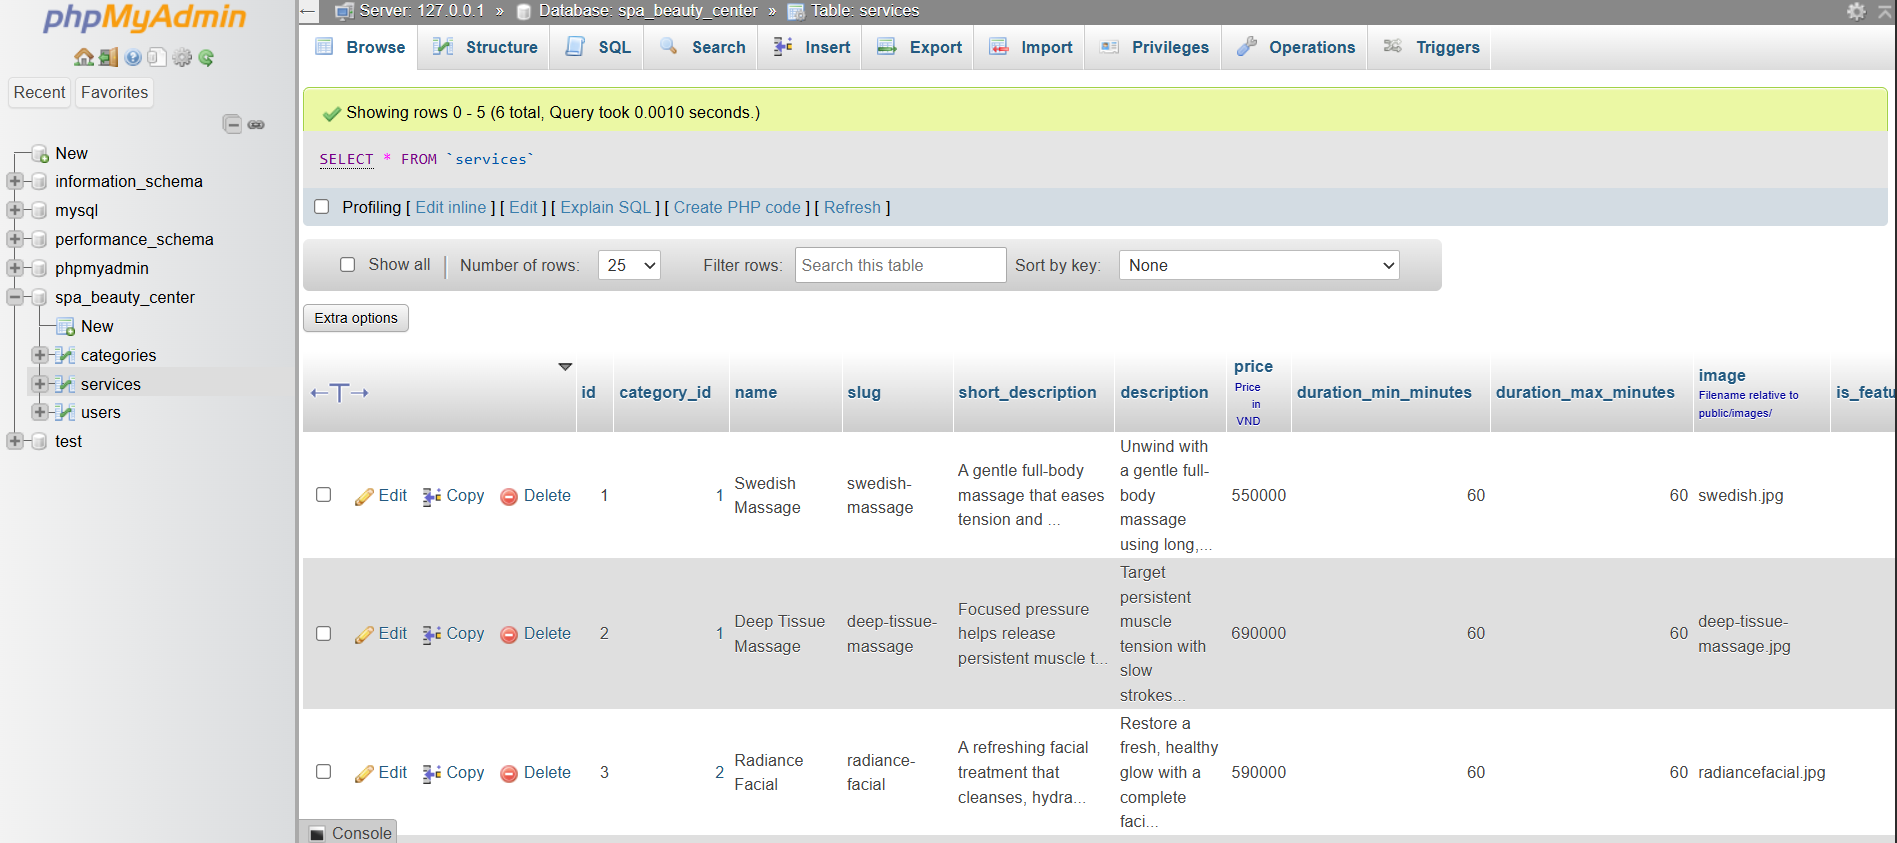
\includegraphics[width=\linewidth,height=0.255\textheight,keepaspectratio]{database-services-evidence.png}
  \captionof{figure}{Service records, including prices, durations, and image filenames.}
  \label{fig:database-services}
\end{minipage}\par\vspace{3mm}

\noindent\begin{minipage}{\linewidth}
  \centering
  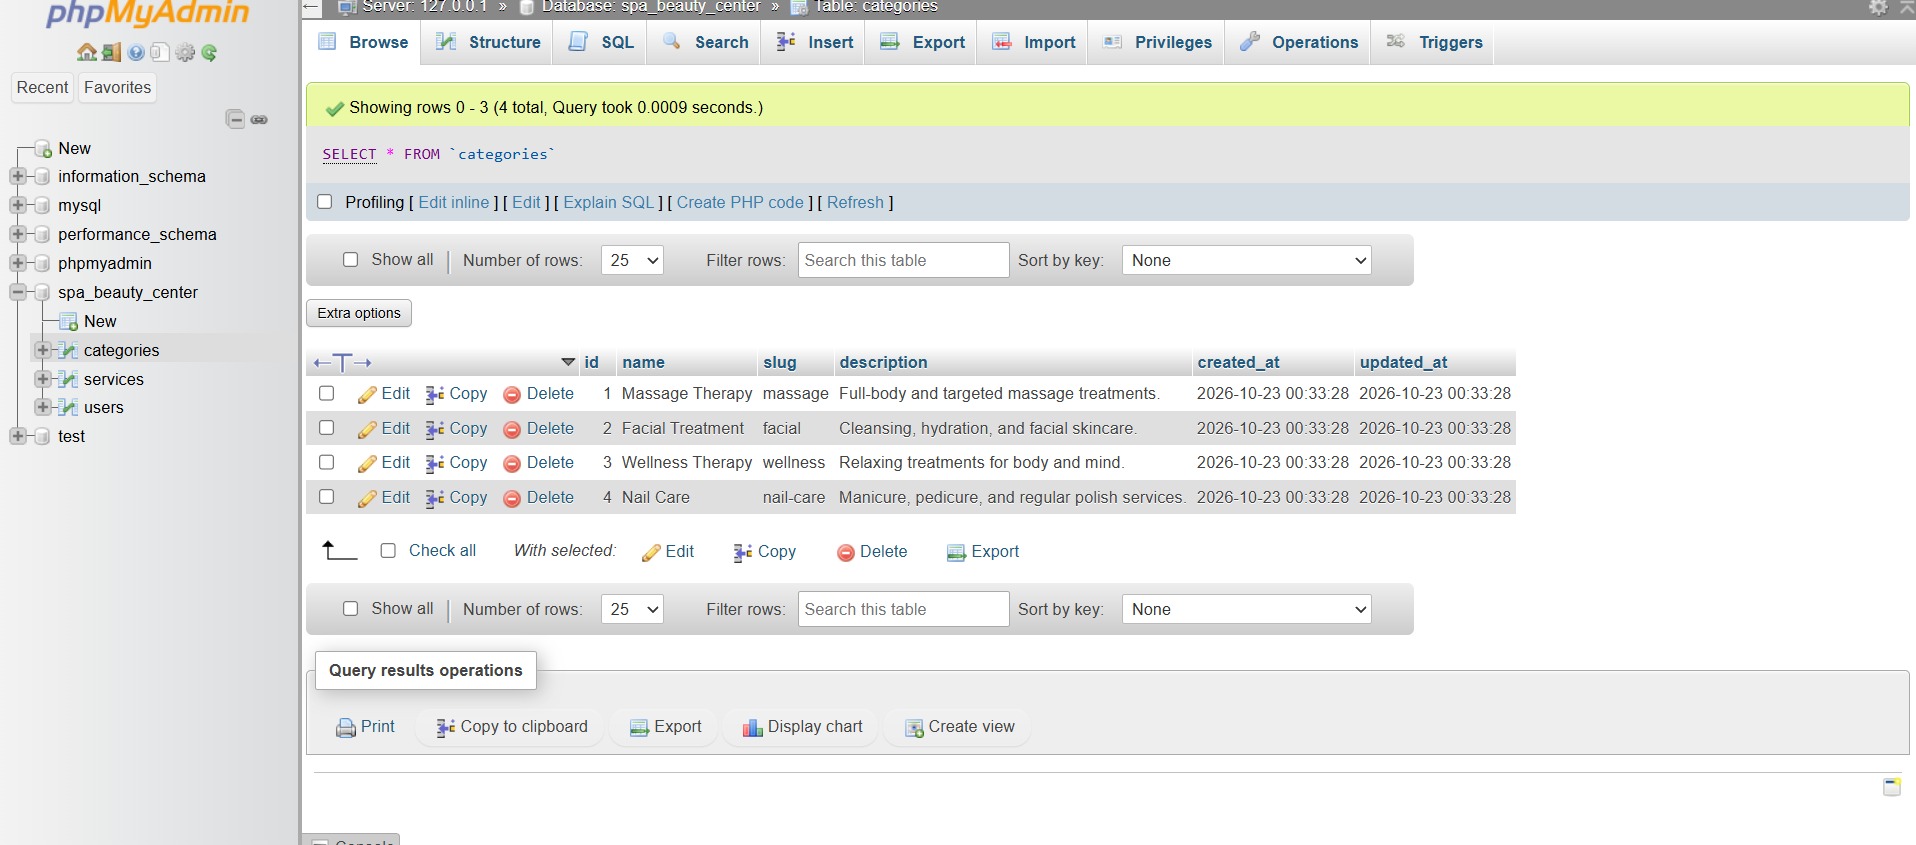
\includegraphics[width=\linewidth,height=0.255\textheight,keepaspectratio]{database-categories-evidence.png}
  \captionof{figure}{The four categories used to organise spa services.}
  \label{fig:database-categories}
\end{minipage}\par\vspace{3mm}

\noindent\begin{minipage}{\linewidth}
  \centering
  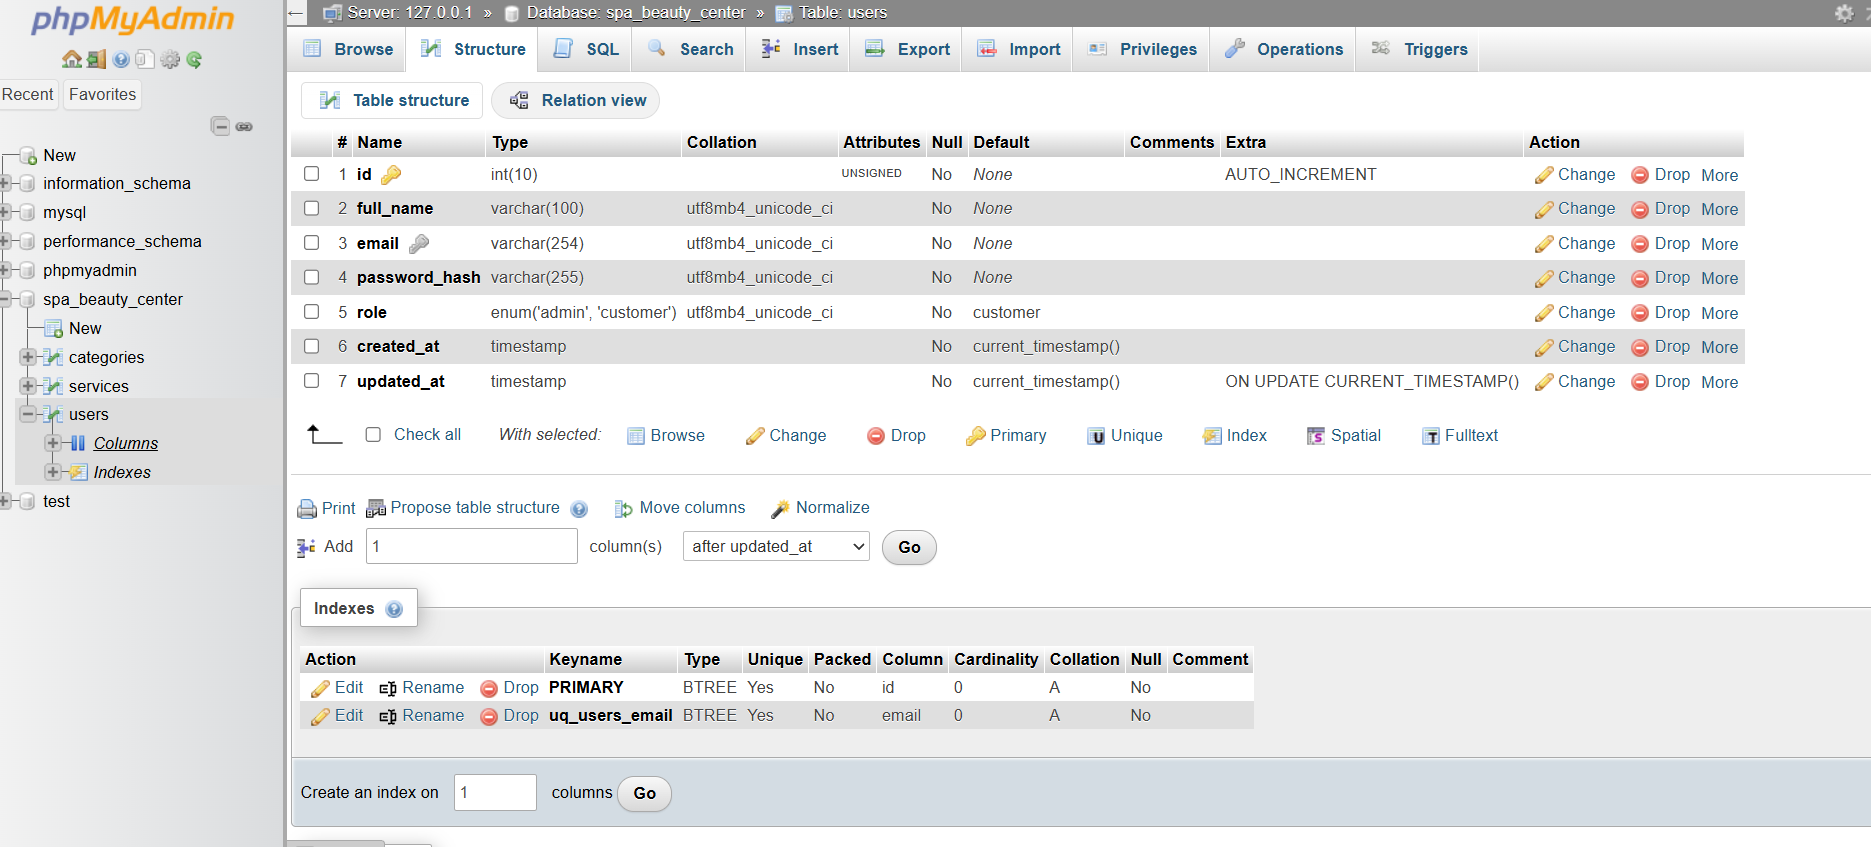
\includegraphics[width=\linewidth,height=0.255\textheight,keepaspectratio]{database-users-structure-evidence.png}
  \captionof{figure}{Users table structure, showing account fields, the password-hash field, roles, and indexes.}
  \label{fig:database-users}
\end{minipage}

\clearpage
\section{Implemented Features}

\subsection{Database Integration (Tasks 1--2)}

The application connects to MariaDB through PHP Data Objects (PDO), with shared
connection settings used across the website. The service catalogue, category
filters, featured treatment, and service details pages retrieve their content
from the database. This allows changes to service records to appear on the
public pages without editing the page markup. If the database is unavailable,
the application displays an error message without exposing connection details
or SQL exceptions. Figures~\ref{fig:task2-mysql-record} and
\ref{fig:task2-website-confirmation} compare a stored service record with its
corresponding details page.

\subsection{Service Management (Task 3)}

The administrator area supports the create, read, update, and delete (CRUD)
operations for services. Administrators can view the service list and individual
records, add treatments, edit existing information, and remove services.
Server-side validation checks required fields, category selections, prices,
durations, slugs, and permitted image filenames. Queries containing user input
use prepared statements. Successful changes are followed by a redirect and a
confirmation message. Deletion requires confirmation and a POST request, and
cross-site request forgery (CSRF) protection is applied to service changes.

\subsection{Registration and Authentication (Task 4)}

Customer registration checks the submitted name and email address, password
requirements, password confirmation, and whether the email address is already
registered. Passwords are stored as hashes using \code{password_hash()} and
checked during login using \code{password_verify()}. After successful login,
customers can access a protected account dashboard. Logout uses a
CSRF-protected request and invalidates the authenticated session.

\subsection{Sessions and Display Preferences (Task 5)}

PHP sessions keep customers authenticated as they move between pages.
A separate cookie stores the selected light or dark appearance. This preference
persists after logout and does not contain account information. Session and
cookie behaviour is described in more detail in Section~\ref{sec:sessions}.

\subsection{Role-Based Access Control (Task 6)}

Access to service management is restricted to administrators. The server checks
the account's current database role whenever a management page or action is
requested. Customers and unauthenticated visitors are therefore denied access
even if they enter a management URL directly or submit a request outside the
normal interface. For this local laboratory deployment, the management area
also accepts requests only from the computer hosting the application.

\clearpage
\section{Session and Cookie Usage}
\label{sec:sessions}

The application uses two cookies with distinct purposes. Authentication data
is held in a server-side session, while the appearance preference is stored
separately in the browser.

\begin{tabularx}{\linewidth}{@{}P{27mm}YY@{}}
\toprule
\textbf{Cookie} & \textbf{Purpose} & \textbf{Lifetime} \\
\midrule
\code{spa_session} & Identifies the server-side session containing the
authenticated user ID, CSRF tokens, and feedback messages.
& Browser-session cookie. Logout destroys the server-side session and expires
the cookie. \\
\code{spa_theme} & Stores either \code{dark} or \code{light} to retain the
chosen appearance.
& 30 days after selection or migration; retained after logout. \\
\bottomrule
\end{tabularx}

The session cookie uses \code{HttpOnly}, which prevents JavaScript from reading
it. The theme cookie remains accessible to JavaScript so that the appearance
toggle can update the preference. Both cookies use \code{SameSite=Lax}; the
\code{Secure} attribute is enabled when the application is served over HTTPS.
The local test environment uses HTTP.

Successful login regenerates the session identifier. Protected requests use the
stored user ID to retrieve the account's current role from the database, so a
role change takes effect on the next request. The theme cookie contains no
passwords, password hashes, or role information and has no effect on access
permissions.

The implementation does not enforce an application-level idle timeout. A
browser-session cookie also does not guarantee logout when a browser restores
previously opened tabs. Explicit logout provides the means of invalidating
the authenticated session.
Figures~\ref{fig:task5-cookie-stored}--\ref{fig:task5-after-logout} show the
preference cookie before and after reload, navigation, and logout.

\clearpage
\section{Testing and Results}

Integration testing for Task 7 used automated tests that
checked database access, service management, authentication, sessions, display
preferences, and access restrictions. Node.js 24.13.1 was used for JavaScript
testing, and a Chrome workflow checked the appearance controls and cookie
behaviour in the browser.

\begin{tabularx}{\linewidth}{@{}P{37mm}YP{24mm}@{}}
\toprule
\textbf{Test area} & \textbf{Coverage} & \textbf{Result} \\
\midrule
Database integration & Connection, catalogue and details pages, malformed
links, and database-outage responses. & 128 checks passed \\
Service management & CRUD operations, changes reflected on public pages,
validation, output escaping, CSRF protection, and deletion confirmation.
& 183 checks passed \\
Authentication and sessions & Registration, unique email addresses, password
hashes, login, session persistence and ID regeneration, logout, and rejection
of invalidated sessions. & 188 checks passed \\
Access control & Rejection of unauthenticated and customer requests,
manipulated role values, administrator actions, role changes, and deleted
accounts. & 310 checks passed \\
Theme preference & Cookie values, persistence, expiry, migration, preference
priority, and behaviour when browser storage is blocked. & 8 tests passed \\
Browser workflow & Theme toggle, cookie expiry and attributes, page reloads,
navigation, initial theme rendering, and invalid-cookie handling. & Passed \\
\bottomrule
\end{tabularx}

The final test run recorded \textbf{809 PHP checks and 8 JavaScript tests
passed}, together with a successful Chrome workflow. Syntax checks also passed
for 27 PHP files and three JavaScript files used by the application and browser
tests. Registration, login, logout, and service management were tested through
HTTP requests to the PHP forms. The Chrome workflow focused on visual behaviour
and cookies; it did not exercise every form through the browser interface.

The test suites were run sequentially through \code{tests/run-lab2.ps1}.
Temporary accounts and services were removed after testing. Before-and-after
comparisons found no changes to the original account and service records, and
the database contained zero users, four categories, and six services both before
and after the run. These checks helped confirm that the tests did not alter the
initial application data.

\section{Problems Encountered and Resolutions}

A review identified a potential timing issue in browser tests that repeatedly
navigated to the same URL.
The test could inspect the previous page before the new document had finished
loading, producing results based on outdated page content. The test was revised
to wait for the new document's load event before checking the page. The combined
test suite was then run again.

A further concern was that the separate test suites used the same development
database. Simultaneous execution could cause temporary test records to
interfere with one another and with the checks on the original data. The
combined runner addresses this by executing the suites in sequence and returning
a failure status if a suite fails.

No failures were reported in the final integrated run. The results cover the
laboratory workflows listed in the testing section; deployment beyond the local
XAMPP environment was outside the scope of this lab. The database, authentication,
and service management features provide a basis for the next stage of the
semester project.

\clearpage
\appendix
\section{Supporting Screenshots}

The following screenshots illustrate the database structure and the main
application workflows described in this report.

\begin{figure}[ht!]
  \centering
  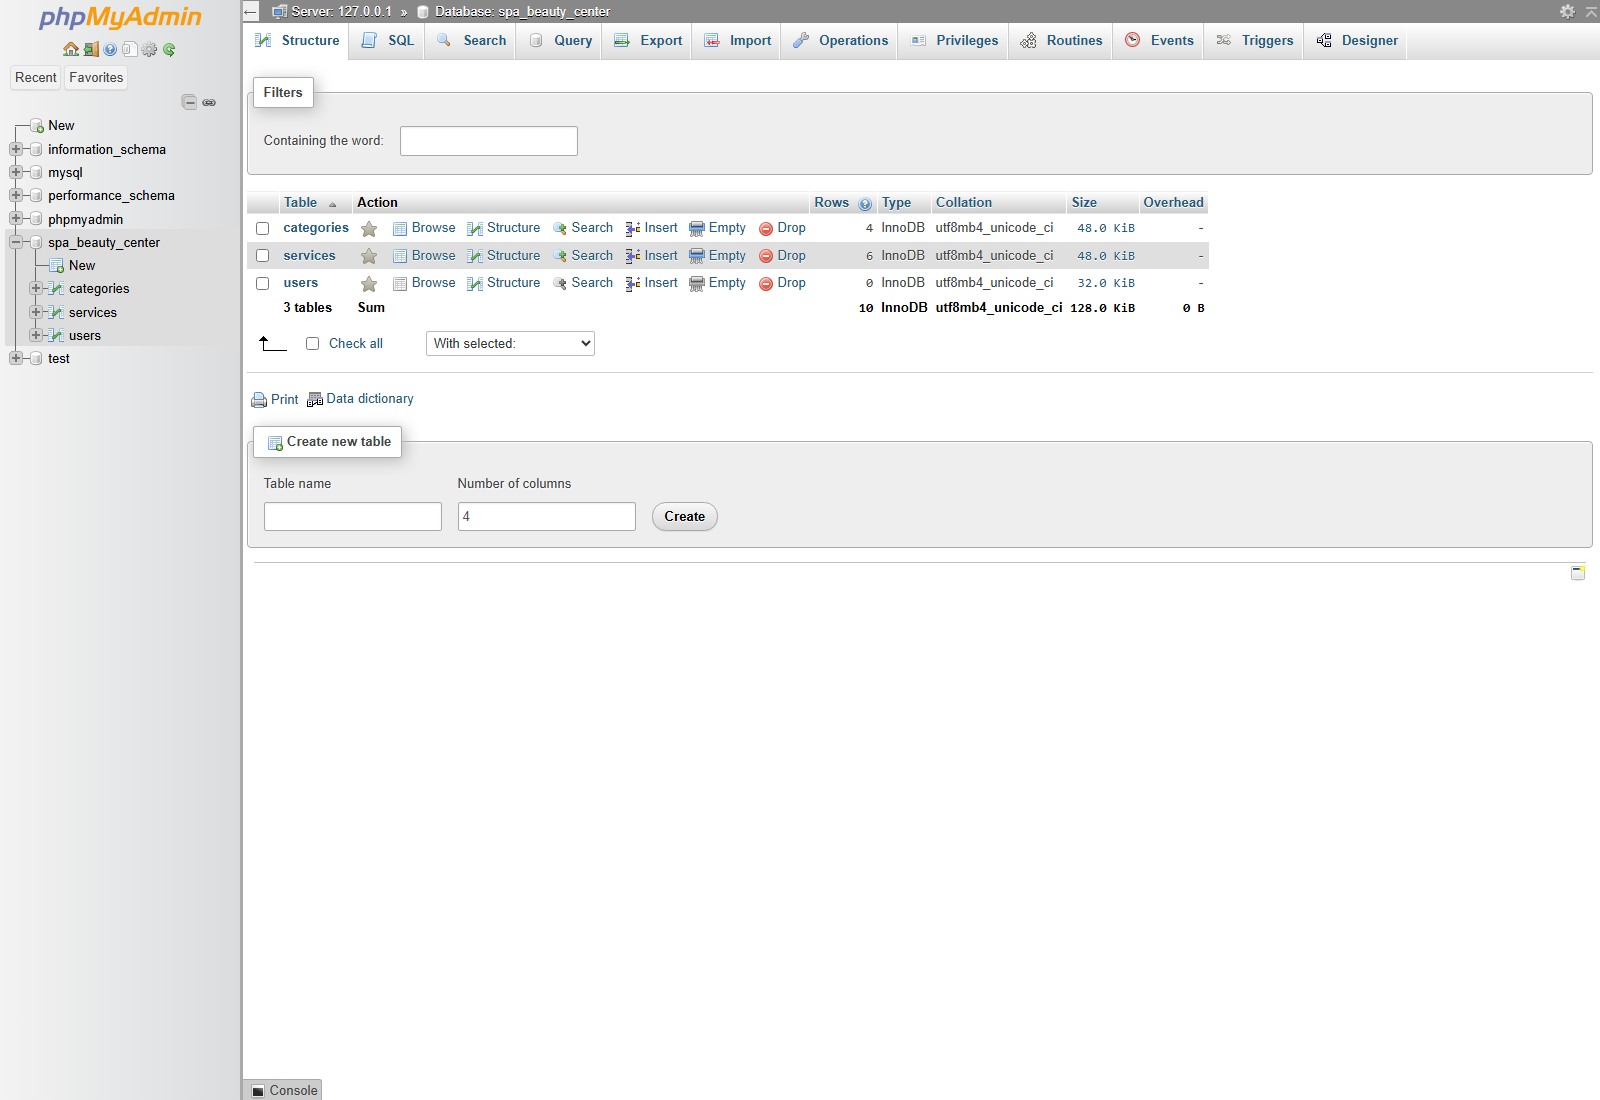
\includegraphics[width=\linewidth,height=0.34\textheight,keepaspectratio]{task1-database-structure.png}
  \caption{Database overview in phpMyAdmin, showing the three application tables.}
\end{figure}

\clearpage
\subsection*{Task 2: Database Content and Website Display}

Figures~\ref{fig:task2-mysql-record} and
\ref{fig:task2-website-confirmation} show the Swedish Massage record in the
database and the information displayed on its details page.

\noindent\begin{minipage}{\linewidth}
  \centering
  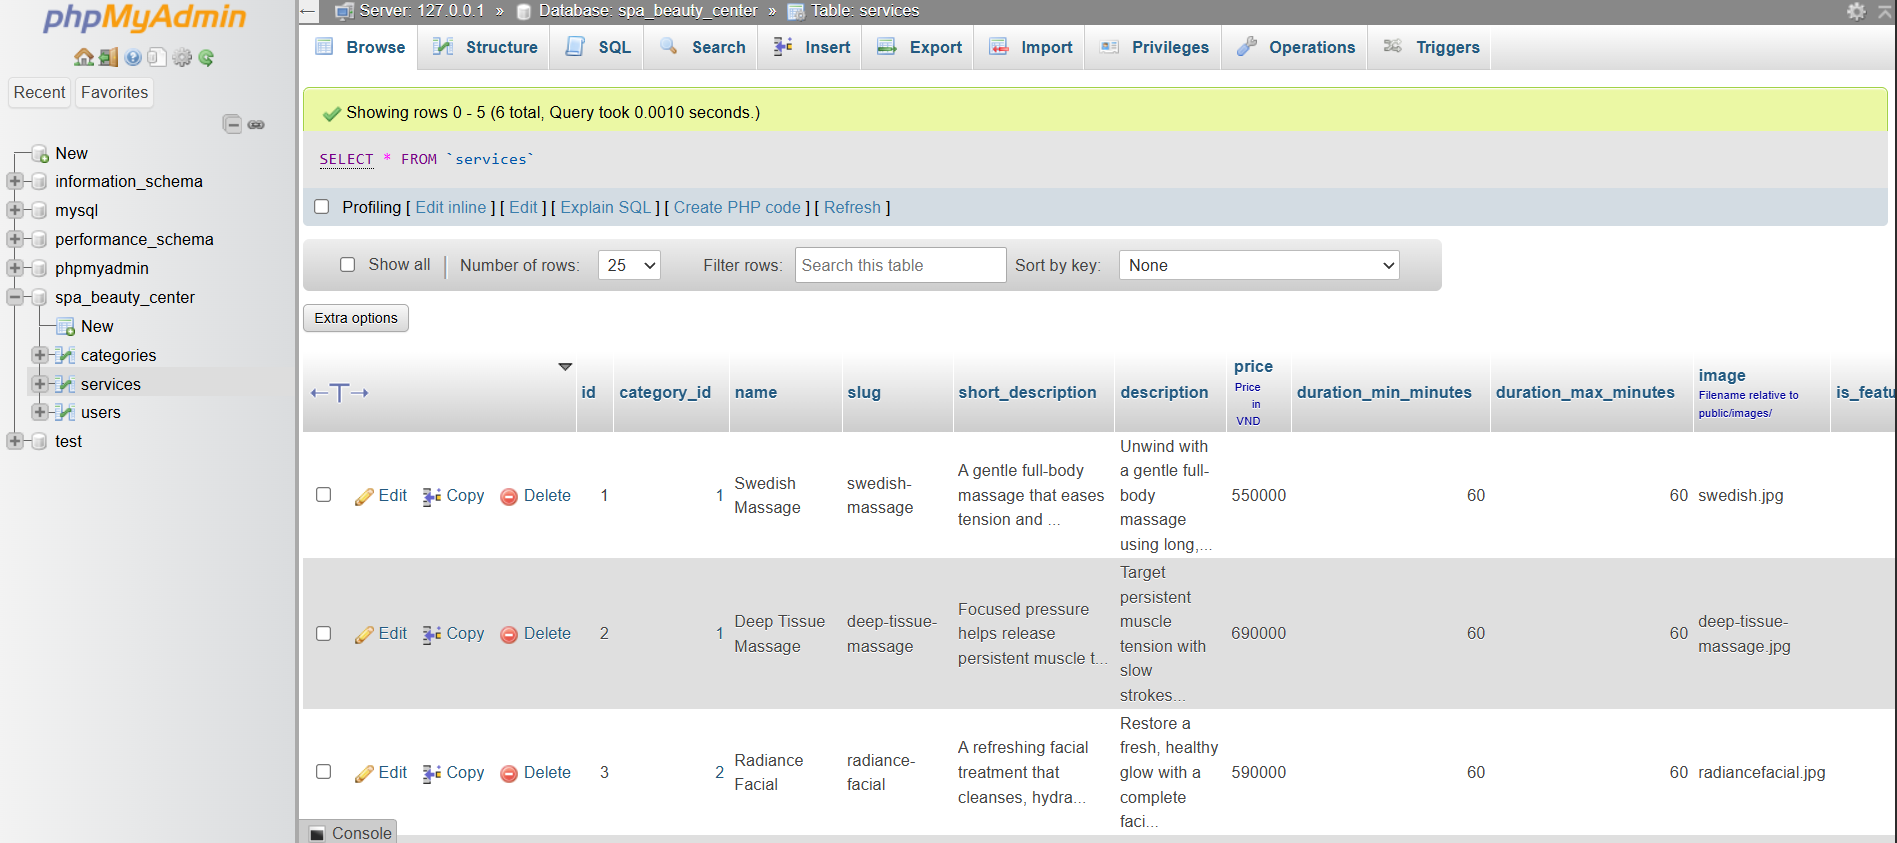
\includegraphics[width=\linewidth,height=0.26\textheight,keepaspectratio]{database-services-evidence.png}
  \captionof{figure}{The Swedish Massage record and its stored values in MariaDB.}
  \label{fig:task2-mysql-record}
\end{minipage}\par\vspace{3mm}

\noindent\begin{minipage}{\linewidth}
  \centering
  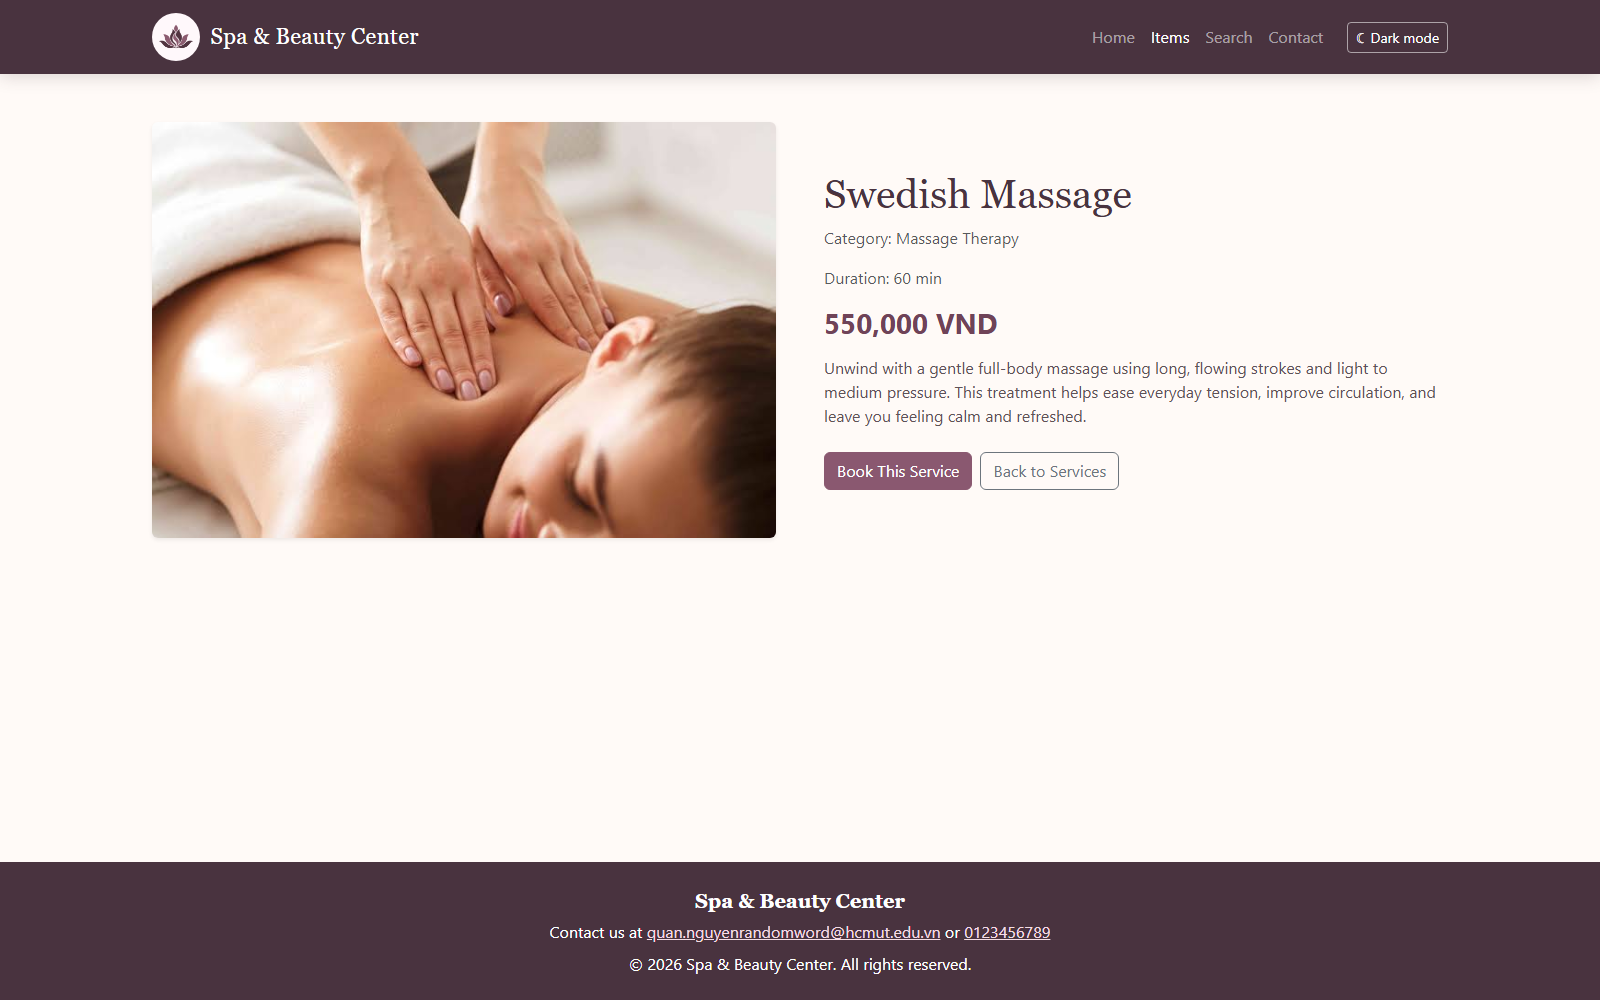
\includegraphics[width=\linewidth,height=0.35\textheight,keepaspectratio]{task2-service-details.png}
  \captionof{figure}{The corresponding Swedish Massage details page.}
  \label{fig:task2-website-confirmation}
\end{minipage}\par\vspace{3mm}

{\small\noindent
\begin{tabularx}{\linewidth}{@{}P{35mm}YY@{}}
\toprule
\textbf{Field} & \textbf{Stored value} & \textbf{Website display} \\
\midrule
Service name & Swedish Massage & Swedish Massage \\
Price & 550000 & 550,000 VND \\
Duration & Minimum 60, maximum 60 minutes & 60 min \\
\bottomrule
\end{tabularx}\par
}

The displayed name, price, and duration match the database record. The website
formats the price with a thousands separator and a currency label while
preserving the stored amount.

\clearpage
\begin{figure}[ht!]
  \centering
  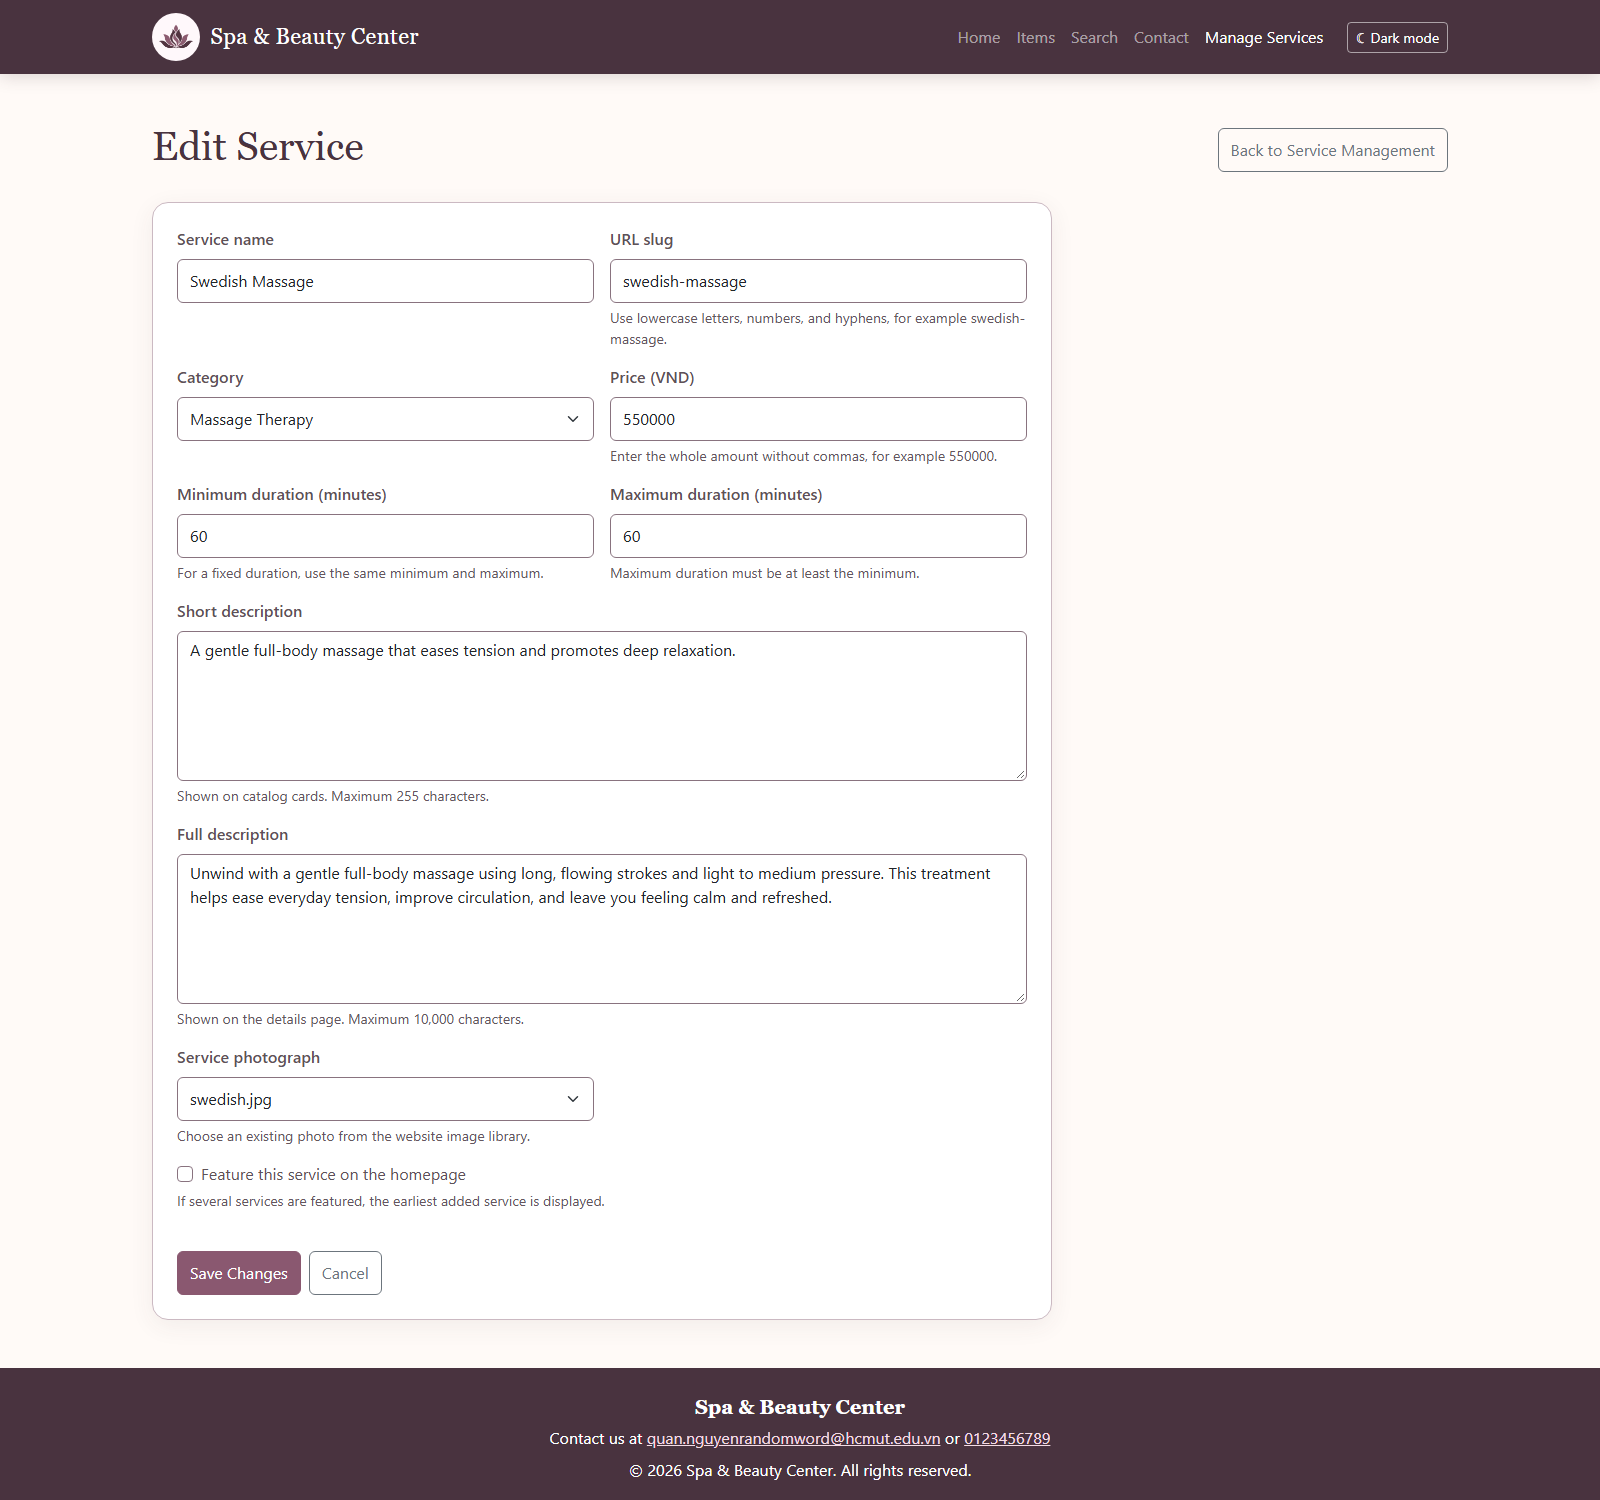
\includegraphics[width=\linewidth,height=0.40\textheight,keepaspectratio]{task3-service-form.png}
  \caption{Administrator form for adding or editing a spa service.}
\end{figure}
\begin{figure}[ht!]
  \centering
  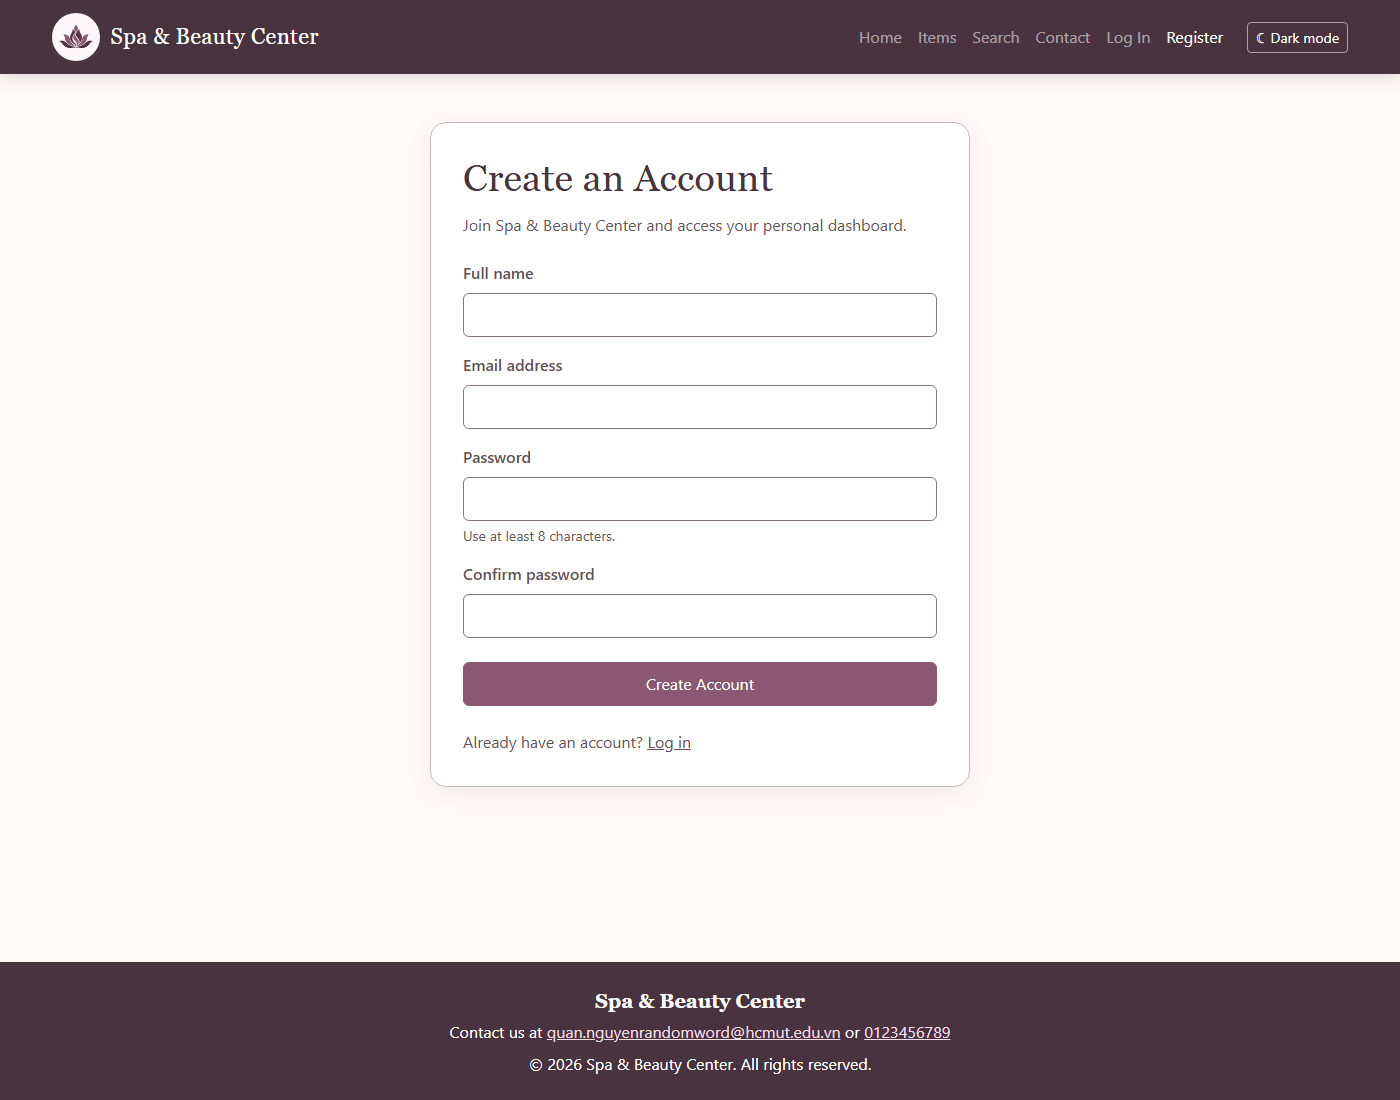
\includegraphics[width=\linewidth,height=0.40\textheight,keepaspectratio]{task4-registration.png}
  \caption{Customer registration form with account details and password confirmation.}
\end{figure}

\clearpage
\begin{figure}[ht!]
  \centering
  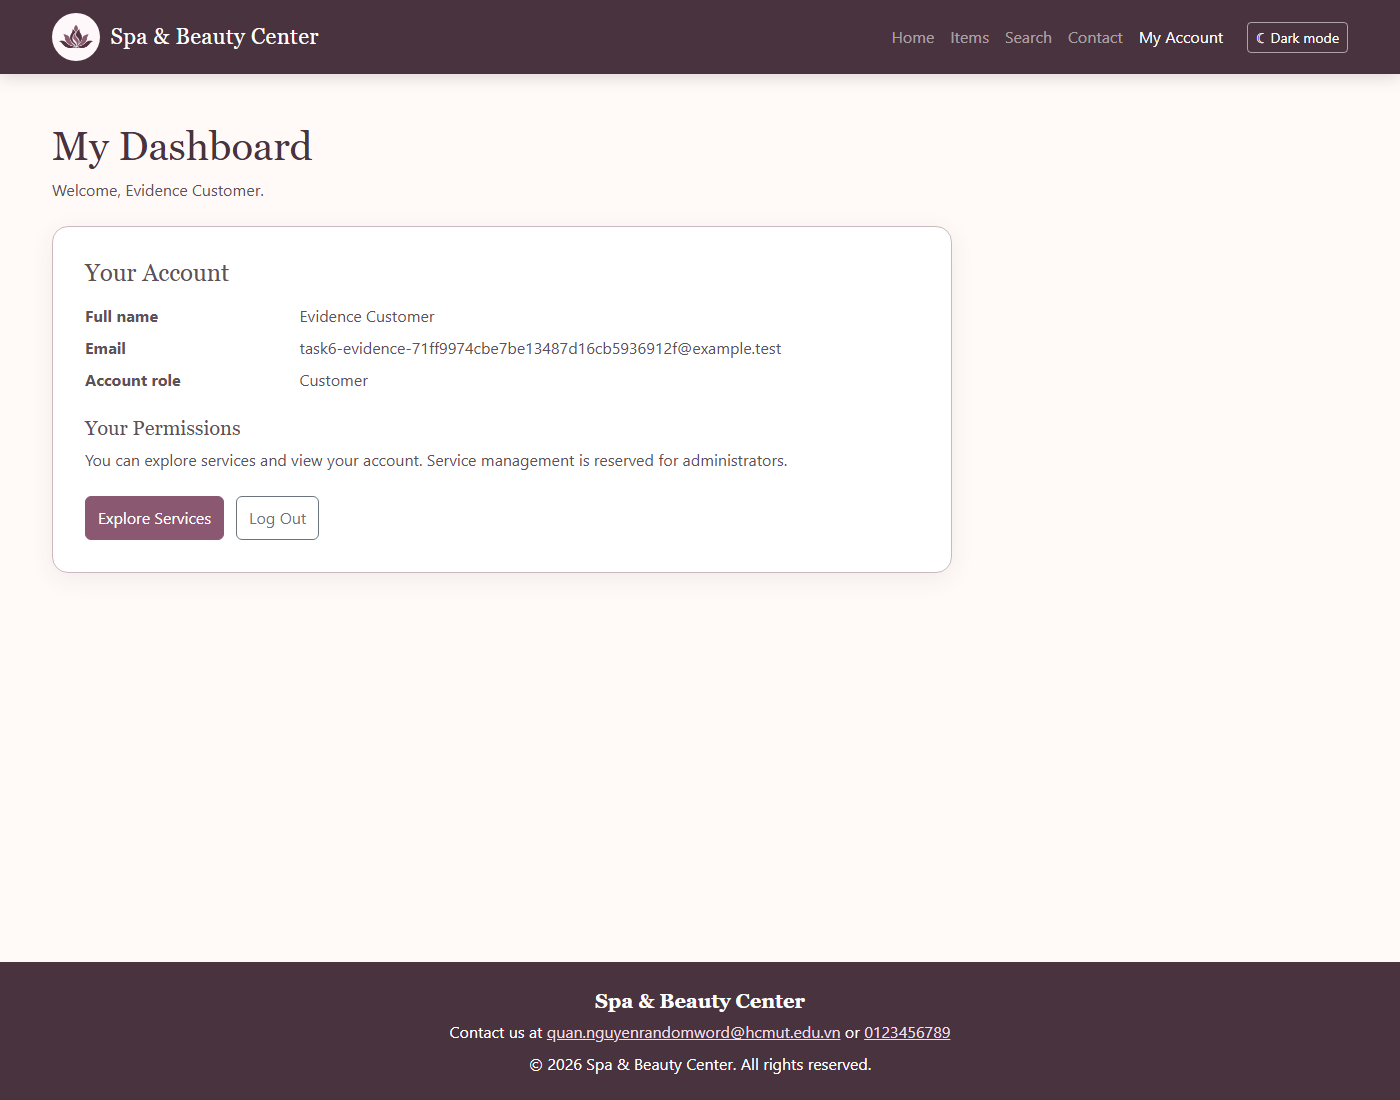
\includegraphics[width=\linewidth,height=0.40\textheight,keepaspectratio]{task6-customer-dashboard.png}
  \caption{Customer dashboard after successful authentication.}
\end{figure}
\begin{figure}[ht!]
  \centering
  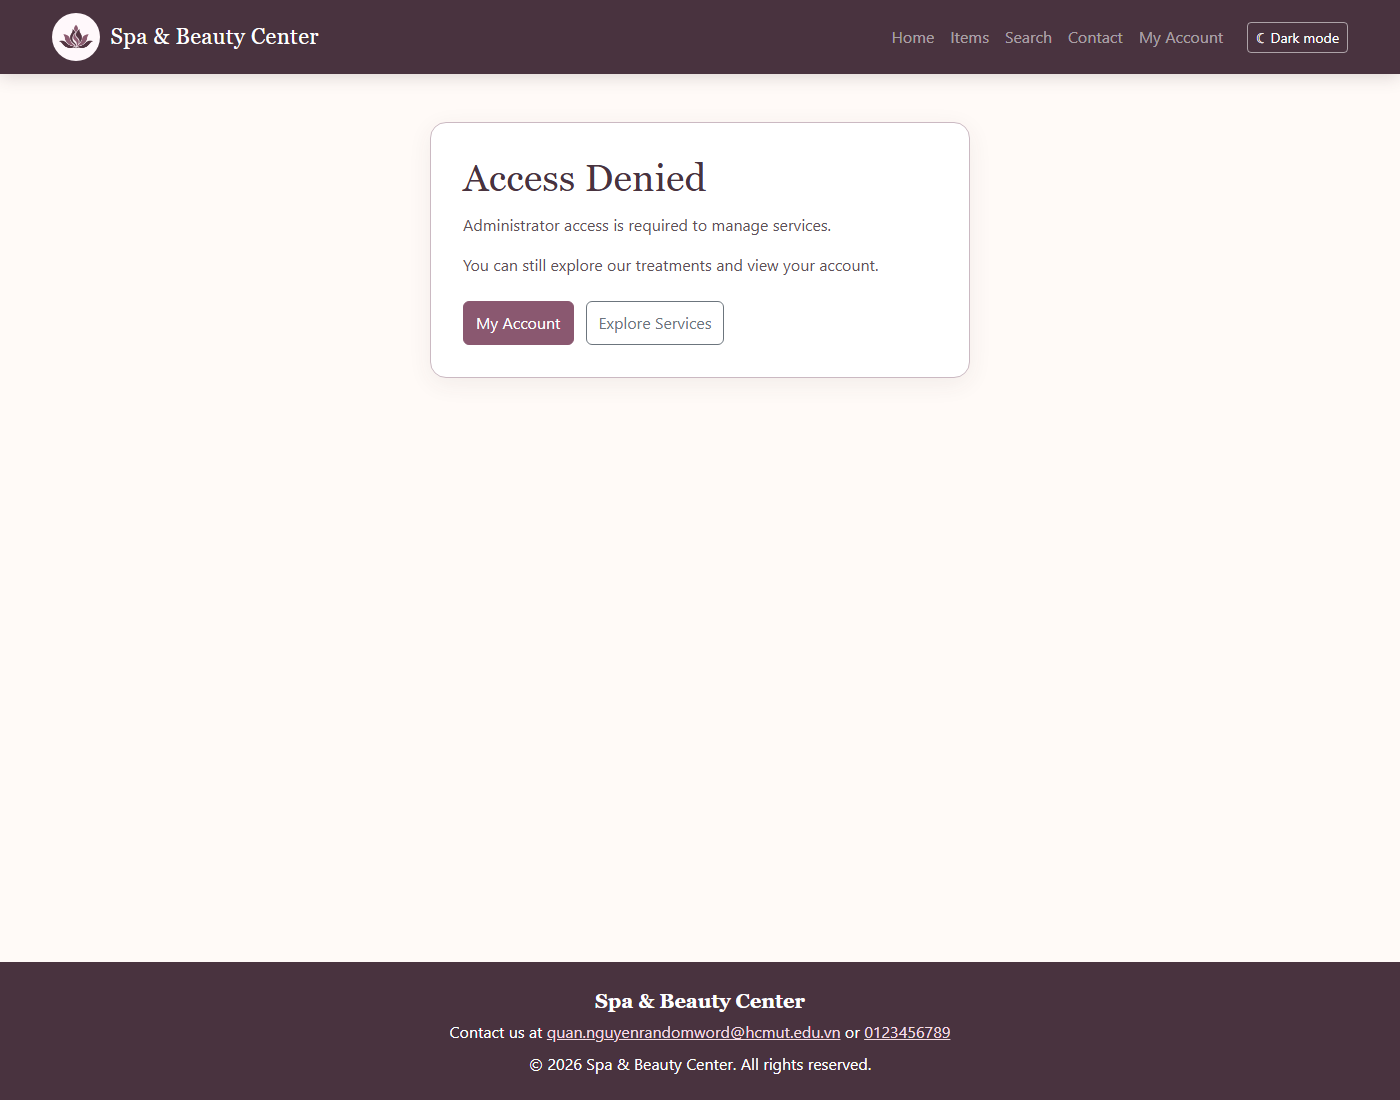
\includegraphics[width=\linewidth,height=0.40\textheight,keepaspectratio]{task6-customer-access-denied.png}
  \caption{Access denied when a customer requests a service management page.}
\end{figure}

\clearpage
\begin{figure}[ht!]
  \centering
  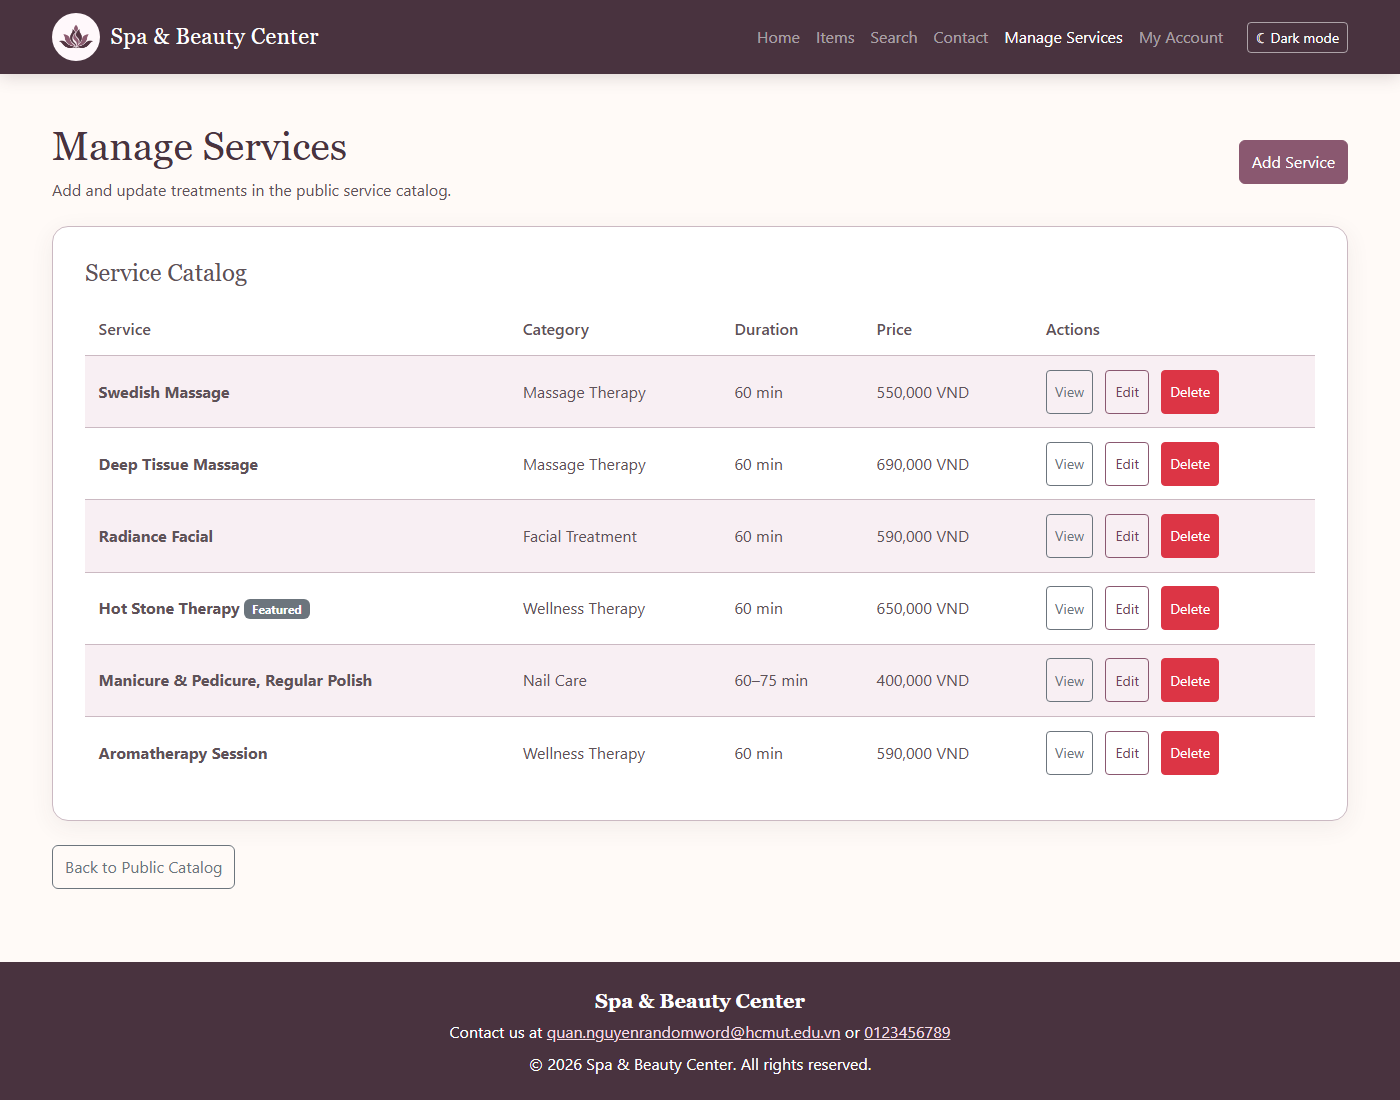
\includegraphics[width=\linewidth,height=0.40\textheight,keepaspectratio]{task6-admin-services.png}
  \caption{Administrator service list with controls to add, view, edit, and delete records.}
\end{figure}

\clearpage
\subsection*{Task 5: Cookie Storage}
The evidence was captured in an isolated Chrome profile. Each pair shows
separate website and native DevTools views of the same browser state; only
\code{spa_theme} is shown in the cookie table. Cookie views focus on the
Application tab, filter, and preference row; original full-resolution
screenshots are retained.

\noindent\begin{minipage}{\linewidth}
  \centering
  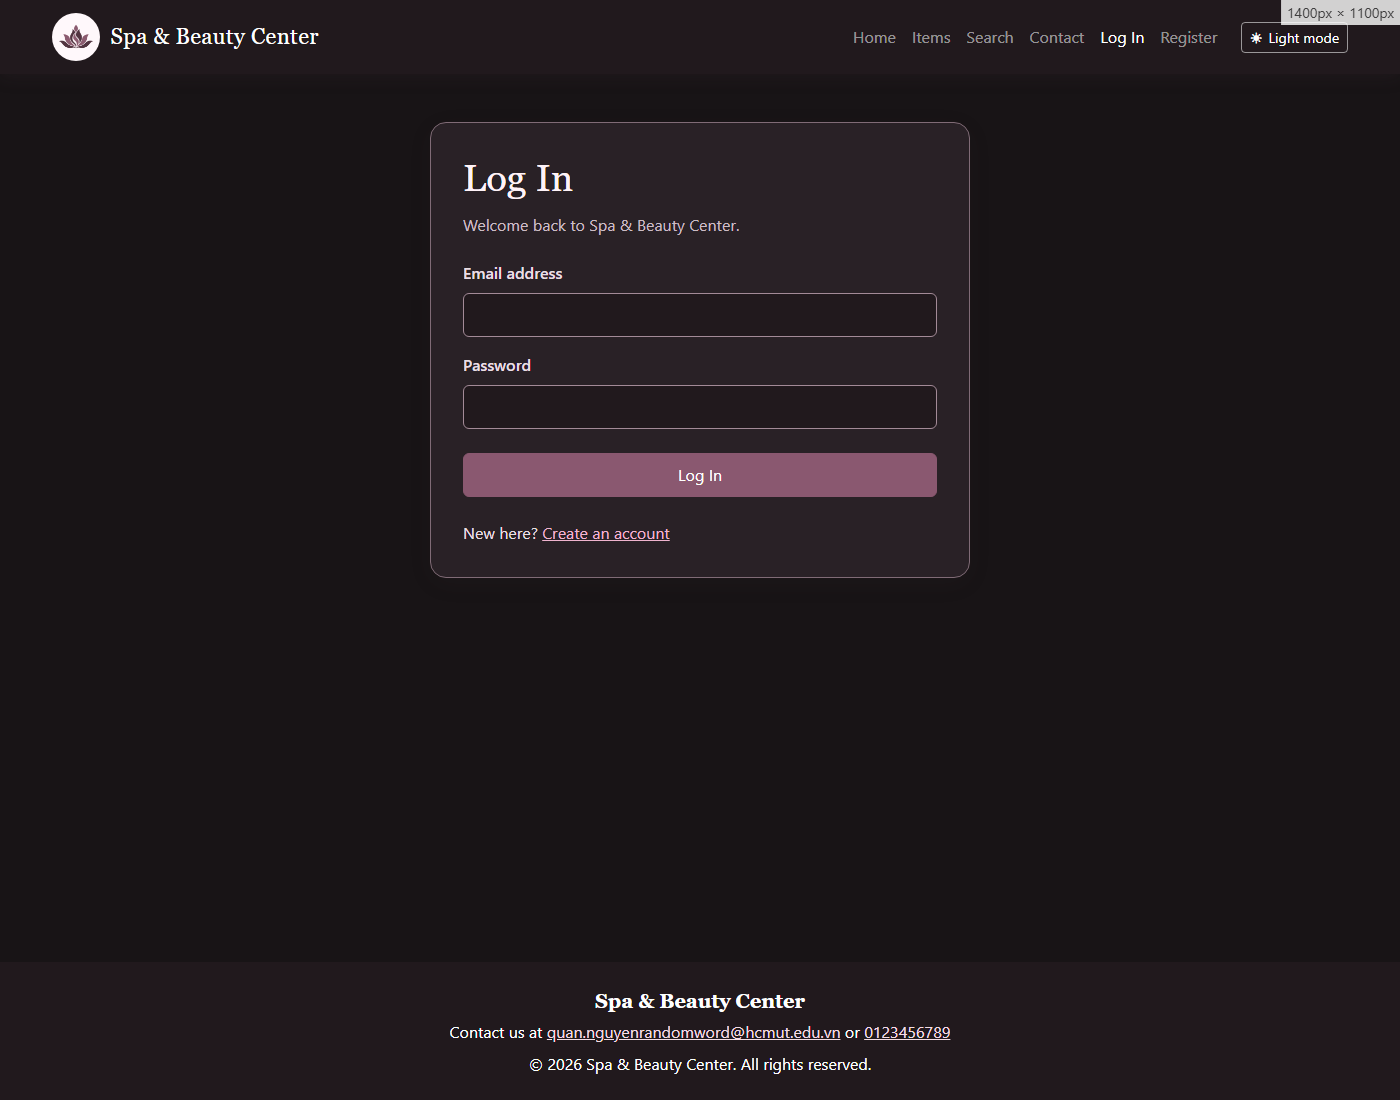
\includegraphics[trim=0bp 480bp 0bp 0bp,clip,width=\linewidth]{task5-page-stored.png}
  \captionof{figure}{Step 1 -- Selecting dark mode writes the appearance preference.}
\end{minipage}\par\vspace{3mm}

\noindent\begin{minipage}{\linewidth}
  \centering
  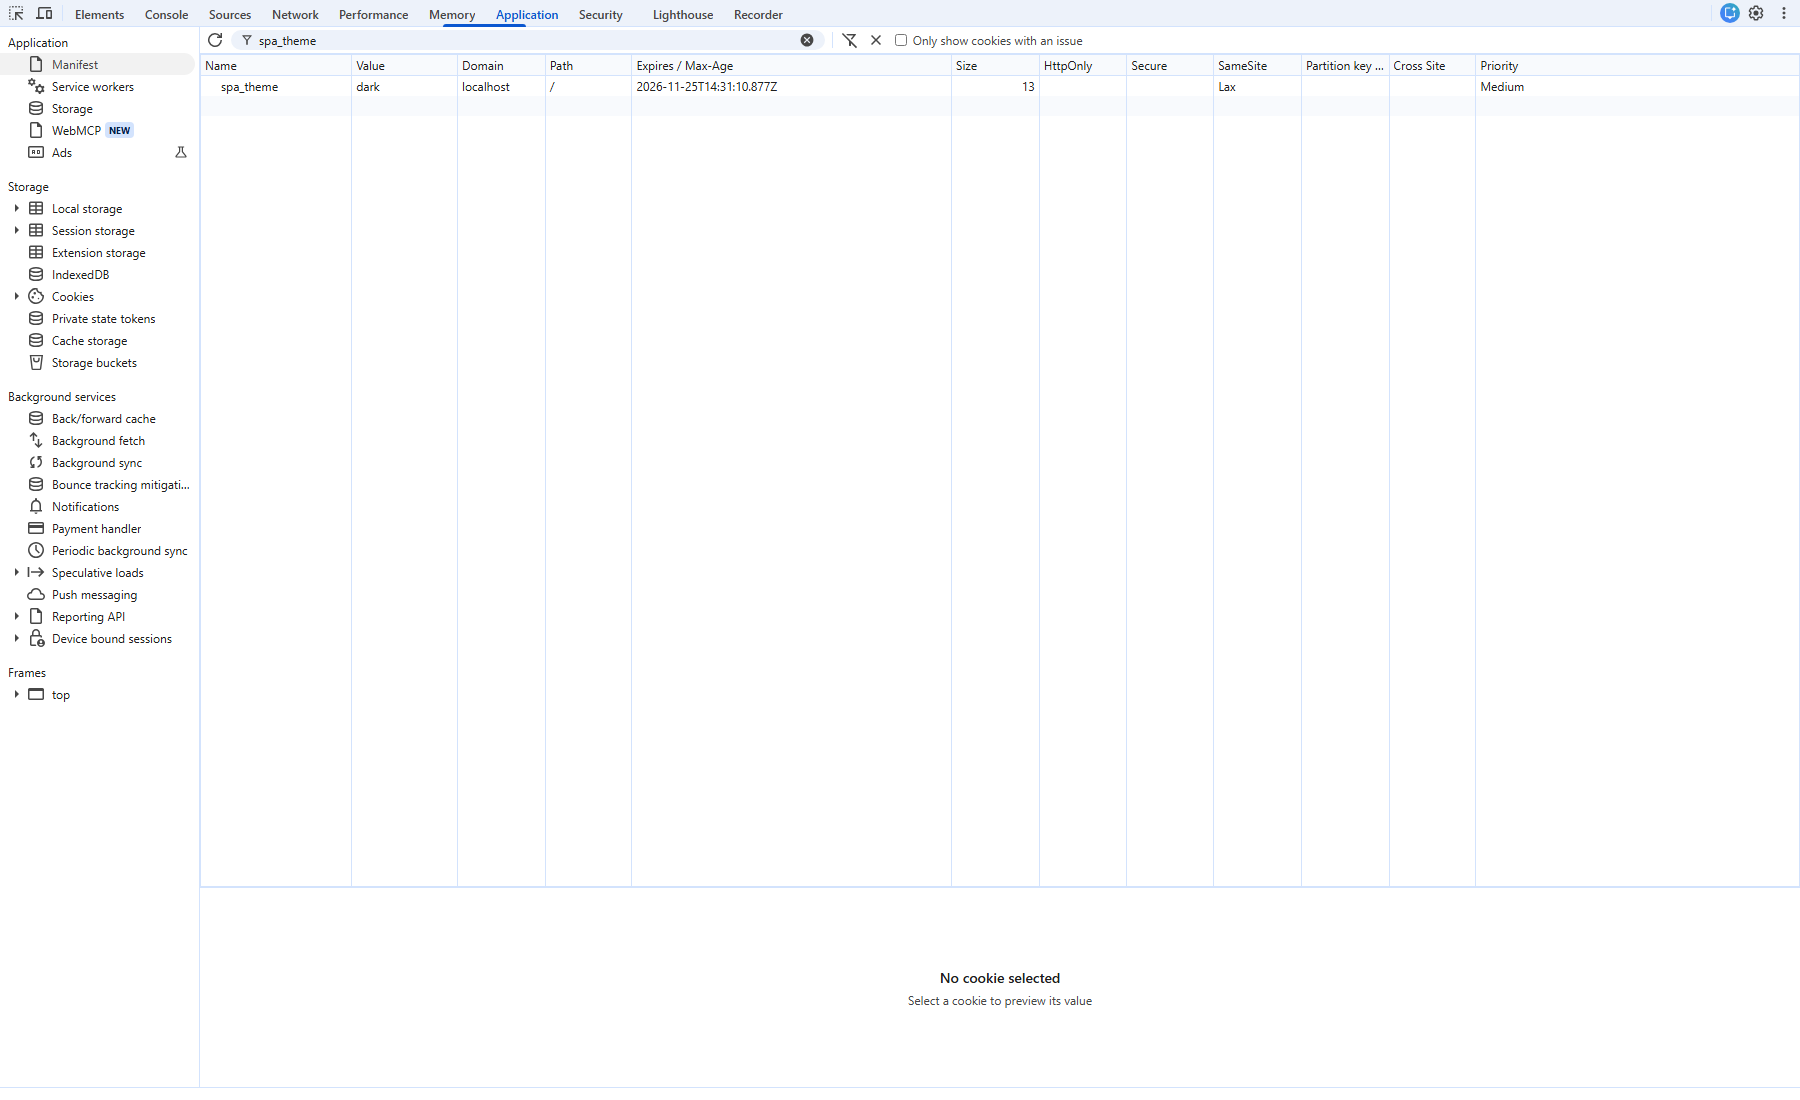
\includegraphics[trim=200bp 980bp 495bp 0bp,clip,width=\linewidth]{task5-cookie-stored.png}
  \captionof{figure}{Native Application/Cookies view: the saved preference and expiry.}
  \label{fig:task5-cookie-stored}
\end{minipage}\par\vspace{3mm}

{\small\noindent
\begin{tabularx}{\linewidth}{@{}P{36mm}Y@{}}
\toprule
\textbf{Attribute} & \textbf{Observed value} \\
\midrule
Name / value & \code{spa_theme} / \code{dark} \\
Domain / path & \code{localhost} / \code{/} \\
Expiry (UTC) & 25 November 2026, 14:31:10.877 \\
Configured lifetime & 2,592,000 seconds (30 days) from selection \\
SameSite & \code{Lax} \\
HttpOnly / Secure & Both false: a JavaScript-readable preference on local HTTP \\
\bottomrule
\end{tabularx}\par}

The expiry is configured for 30 days; this capture does not claim observation
over 30 elapsed days. The cookie contains no account identity or credentials.

\clearpage
\subsection*{Task 5: Reload and Navigation}
The collector reloaded the page, confirmed that dark mode was restored, then
navigated to the Swedish Massage details page in the same browser profile.

\noindent\begin{minipage}{\linewidth}
  \centering
  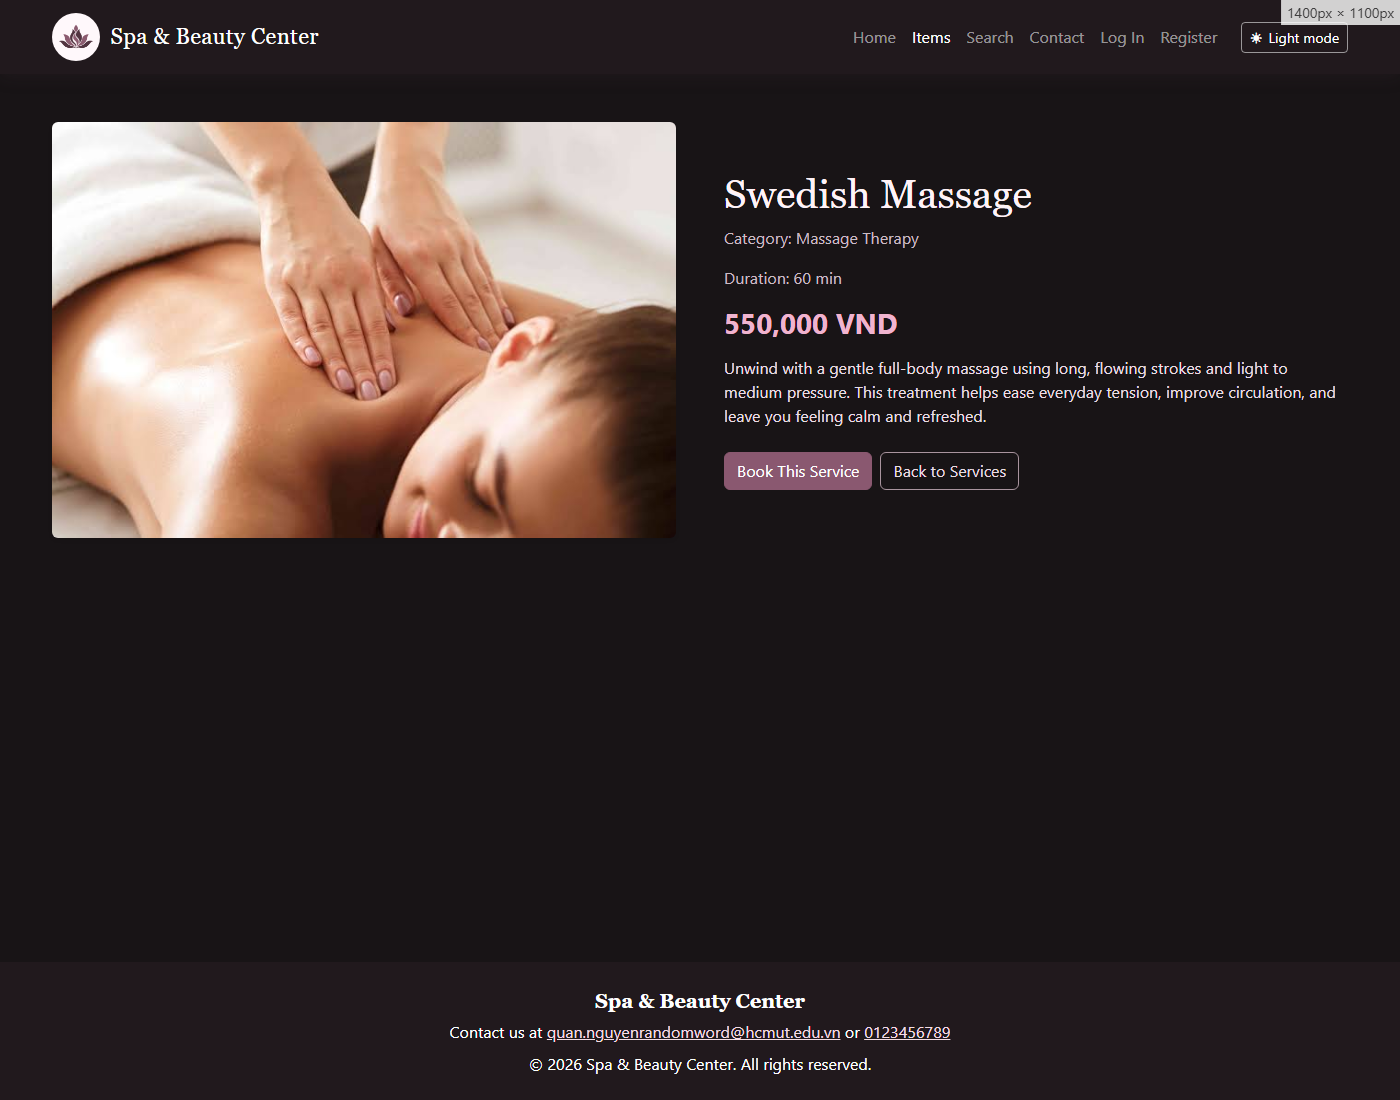
\includegraphics[trim=0bp 480bp 0bp 0bp,clip,width=\linewidth]{task5-page-persisted.png}
  \captionof{figure}{Step 2 -- Dark mode remains active on the service details page.}
\end{minipage}\par\vspace{3mm}

\noindent\begin{minipage}{\linewidth}
  \centering
  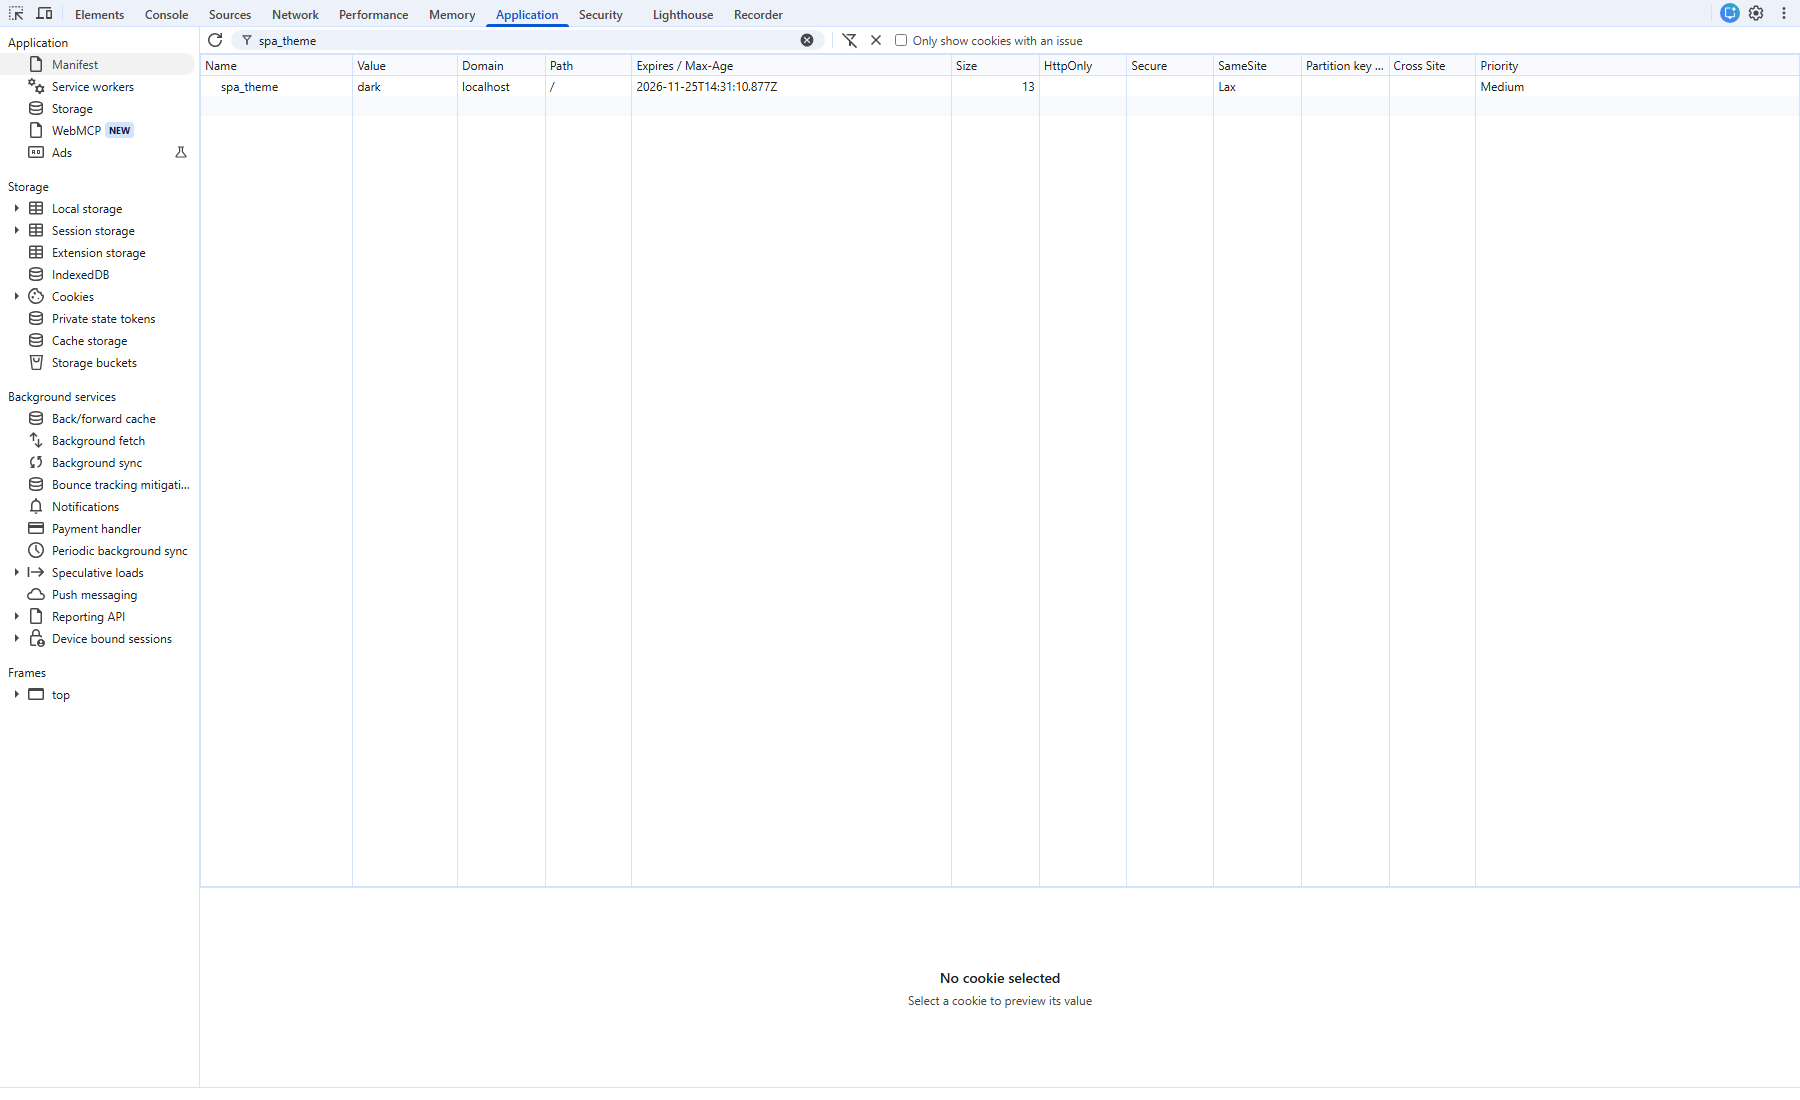
\includegraphics[trim=200bp 980bp 495bp 0bp,clip,width=\linewidth]{task5-cookie-persisted.png}
  \captionof{figure}{After reload/navigation, the preference and original expiry are unchanged.}
  \label{fig:task5-reload-details}
\end{minipage}\par\vspace{3mm}

{\small\noindent
\begin{tabularx}{\linewidth}{@{}P{36mm}YY@{}}
\toprule
\textbf{Check} & \textbf{Before} & \textbf{After reload/navigation} \\
\midrule
Preference & \code{dark} & \code{dark} \\
Expiry (UTC) & 25 Nov 2026, 14:31:10.877 & 25 Nov 2026, 14:31:10.877 \\
Seconds remaining & 2,592,000 & 2,591,997 \\
\bottomrule
\end{tabularx}\par}

The remaining lifetime decreases as time passes. Reloading or opening another
page does not reset the expiry. The collector compared the exact cookie value
and expiry returned by Chrome, not just the visible page colors.

\clearpage
\subsection*{Task 5: Preference After Logout}
A temporary customer registered and logged in through the normal PHP forms.
Login rotated the session identifier. After the CSRF-protected logout,
requesting the protected dashboard redirected to the login page shown below.

\noindent\begin{minipage}{\linewidth}
  \centering
  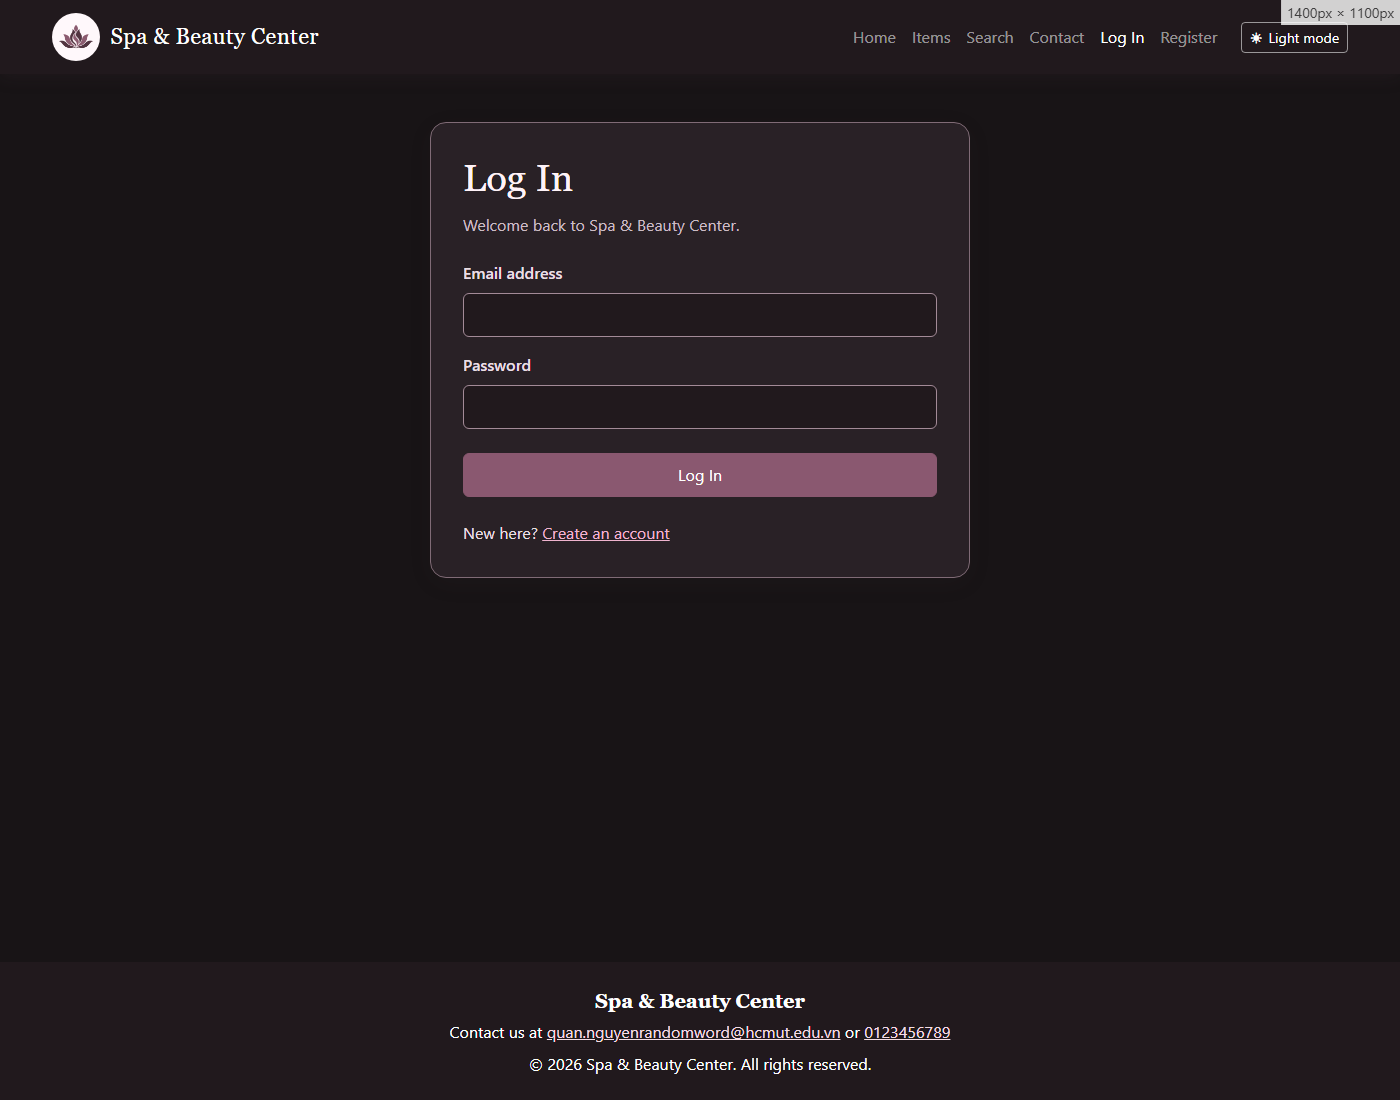
\includegraphics[trim=0bp 480bp 0bp 0bp,clip,width=\linewidth]{task5-page-after-logout.png}
  \captionof{figure}{Step 3 -- Authentication has ended, but the login page stays dark.}
\end{minipage}\par\vspace{3mm}

\noindent\begin{minipage}{\linewidth}
  \centering
  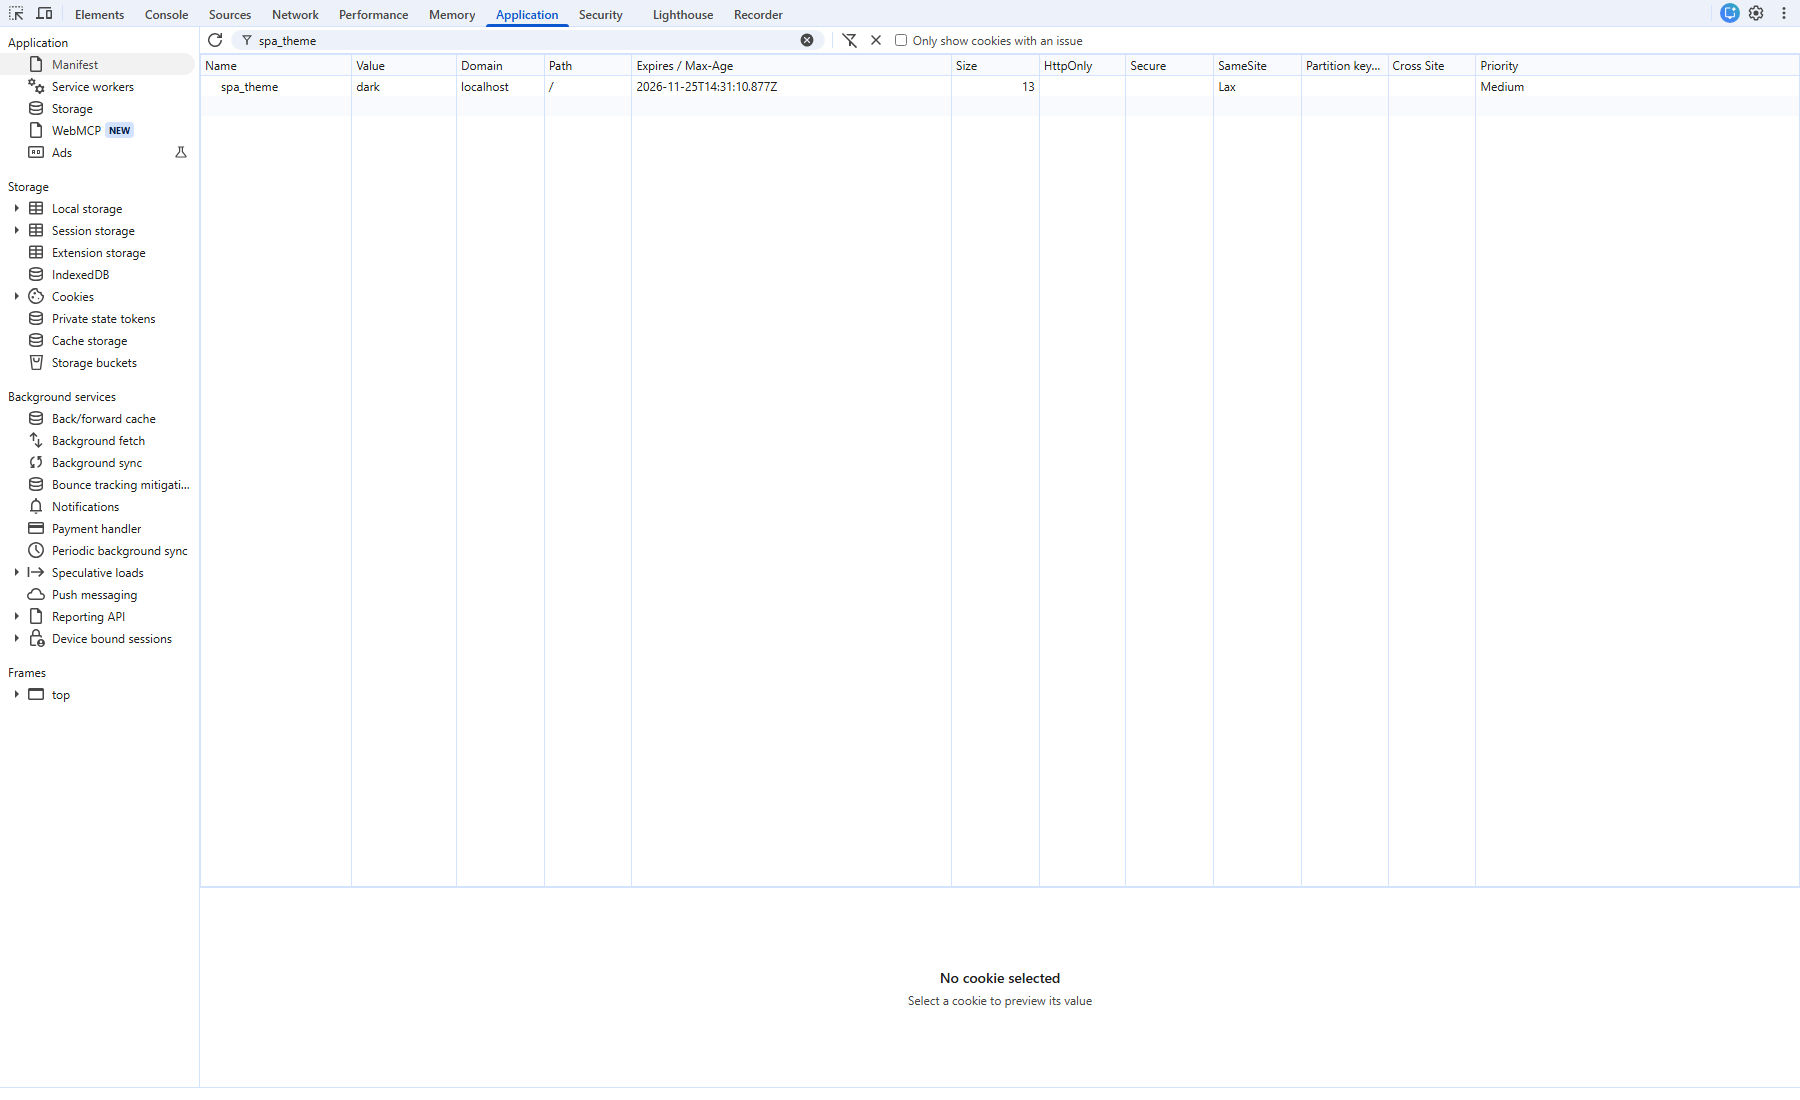
\includegraphics[trim=200bp 980bp 495bp 0bp,clip,width=\linewidth]{task5-cookie-after-logout.png}
  \captionof{figure}{The independent preference cookie survives logout with its original expiry.}
  \label{fig:task5-after-logout}
\end{minipage}\par\vspace{3mm}

The cookie remains \code{spa_theme=dark}, expiring on 25 November 2026 at
14:31:10.877 UTC (2,591,992 seconds remaining at the final check).
The authentication session ends independently of this cosmetic preference.
The login page may create a fresh anonymous session for CSRF protection;
logout does not require the browser to contain no session cookie at all.

Session identifiers, passwords, and CSRF values are excluded from the captures.
The temporary account and isolated browser profile were removed after the
successful capture. Safe cookie attributes are recorded in
\code{docs/screenshots/task5-cookie-metadata.json}.

\end{document}
